\pdfoutput=1
\documentclass[11pt]{amsart}

\usepackage{amsmath,amssymb,amsthm}
\usepackage[margin=1.2in]{geometry}
\usepackage{booktabs}
\usepackage{adjustbox}
\usepackage{xcolor}
\usepackage{tikz}
\usetikzlibrary{arrows.meta}
\usepackage[colorlinks=true,linkcolor=blue,citecolor=blue,urlcolor=blue]{hyperref}
\hypersetup{pdfauthor={Bernd Johannes Wuebben},
  pdftitle={Harmonic paths and honeycombs}}
\setlength{\emergencystretch}{2em}

\newtheorem{theorem}{Theorem}[section]
\newtheorem{proposition}[theorem]{Proposition}
\newtheorem{lemma}[theorem]{Lemma}
\newtheorem{corollary}[theorem]{Corollary}
\theoremstyle{definition}
\newtheorem{definition}[theorem]{Definition}
\newtheorem{example}[theorem]{Example}
\newtheorem{question}[theorem]{Question}
\theoremstyle{remark}
\newtheorem{remark}[theorem]{Remark}

\newcommand{\RR}{\mathbb R}
\newcommand{\CC}{\mathbb C}
\newcommand{\NN}{\mathbb N}
\newcommand{\OO}{\mathcal O}
\newcommand{\mm}{\mathfrak m}
\newcommand{\GL}{\operatorname{GL}}
\newcommand{\id}{\operatorname{id}}
\newcommand{\gr}{\operatorname{gr}}
\newcommand{\rk}{\operatorname{rk}}
\newcommand{\Span}{\operatorname{span}}
\newcommand{\sech}{\operatorname{sech}}
\newcommand{\arsinh}{\operatorname{arsinh}}
\newcommand{\midpt}{\operatorname{mid}}
\newcommand{\diam}{\operatorname{diam}}
\newcommand{\Lip}{\operatorname{Lip}}
\newcommand{\Ndiag}{\mathcal N_{\mathrm{diag}}}
\newcommand{\Nall}{\mathcal N}
\newcommand{\Dord}{\mathcal D}
\newcommand{\calQ}{\mathcal Q}
\newcommand{\calY}{\mathcal Y}
\newcommand{\dd}{\mathrm d}
\newcommand{\eps}{\varepsilon}
\newcommand{\norm}[1]{\left\lVert #1\right\rVert}

\title{Harmonic paths and honeycombs}
\author{Bernd Johannes Wuebben}
\subjclass[2020]{16G20 (primary); 12J25, 51E24, 49J45 (secondary)}
\keywords{Harmonic norms, quiver representations, Novikov field, Euclidean
buildings, spectral networks, honeycombs}
\date{November 4, 2026}

\begin{document}
\begin{abstract}
We construct harmonic paths of non-expansive norms on the identity
representation of the $A_2$ quiver from arbitrary triples of diagonalizable
boundary norms over the real-exponent Novikov field. We use symmetric
central charges and a fixed radial area form on the plane. In every finite
rank, the path has a finite apartment presentation and a finite honeycomb
support with actual semistable edge labels and compatible filtrations at
its vertices. It is unique among paths with such presentations whose
one-sided norm motions agree to first order at each join. The construction
minimizes a renormalized convex action. Its algebraic regularity follows
from fixed orthogonal subspaces at gaps in the spectral velocities,
second-order scalar approximations, and descent of finite norm data from
the Hahn field. Repeated boundary spectra and collapsed edges are included.
The result gives existence in the honeycomb specialization of the harmonic-path
conjecture of Haiden--Katzarkov--Kontsevich--Pandit, with uniqueness under an
explicit matching condition absent from the printed edgewise definition.
\end{abstract}
\maketitle

\section{Introduction}\label{sec:introduction}

A triple of non-Archimedean norms contains more information than the
three relative spectral lists. The harmonic-path problem of
Haiden--Katzarkov--Kontsevich--Pandit asks for a geometric reconstruction
that retains this additional information: a path of non-expansive norms
whose spectral velocities trace a labelled network in the plane
\cite[\S\S7.2--7.3]{HKKP26}. We construct such paths for the identity
representation of the $A_2$ quiver, for every full boundary triple and in
every finite rank. The principal point is finite algebraic regularity of
a variational minimum in a completed norm space. A separate converse
identifies that minimum among paths satisfying an explicit first-order
matching condition.

\subsection{The boundary problem}
Let $K$ be the real-exponent Novikov field over the trivially valued field
$\CC$. Thus its elements are formal sums
\[
 f=\sum_{\lambda\in\RR}a_\lambda T^\lambda
\]
whose support is bounded below and has finite intersection with
$(-\infty,b]$ for every $b\in\RR$. For $f\ne0$ set
$\nu(f)=\min\{\lambda:a_\lambda\ne0\}$ and $|f|=e^{-\nu(f)}$.
We write $\OO=\{|f|\le1\}$ and $\mm=\{|f|<1\}$; the residue field is
$\OO/\mm=\CC$. This field is complete but not spherically complete.
Its spherically complete Hahn extension will be used in the proof; the
path constructed by the theorem is defined over $K$.

Fix $V=K^n$ and consider the quiver with one arrow from its vertex $C$
to its vertex $A$. We use the representations
\begin{equation}\label{eq:ABC}
 A=(0\longrightarrow K),\qquad
 B=(K\xrightarrow{\id}K),\qquad
 C=(K\longrightarrow0),\qquad E=B^n,
\end{equation}
and the central charges
\begin{equation}\label{eq:charges}
 Z(A)=e^{\pi i/6},\qquad Z(B)=i,\qquad Z(C)=e^{5\pi i/6}.
\end{equation}
A norm $h$ on $V$ is \emph{diagonalizable}, or \emph{split}, if there are
a basis $e_1,\ldots,e_n$ and real weights $w_1,\ldots,w_n$ such that
\begin{equation}\label{eq:splitnorm}
 h\Bigl(\sum_i b_i e_i\Bigr)=\max_i e^{w_i}|b_i|.
\end{equation}
The norms diagonalized by a fixed basis form an apartment. We retain their
scales; norms are not taken modulo multiplication by a positive scalar.
Two split norms admit a common orthogonal basis. Their $d_2$ distance
is the Euclidean norm of the differences of their logarithmic weights
in such a basis. In particular, this is the unnormalized metric, including
the determinant direction.

A norm on $E$ is a pair $c=(c_A,c_C)$. The identity arrow is non-expansive
exactly when
\begin{equation}\label{eq:order}
 c_A\le c_C
\end{equation}
pointwise on $V$. For a split norm $h$, put
$\overline V_h=\{h\le1\}/\{h<1\}$. A non-expansive pair induces an
arrow $\overline V_{c_C}\to\overline V_{c_A}$ over $\CC$.
The harmonicity condition for a norm in \cite[Definition~7.3]{HKKP26}
is semistability of this reduced representation. Every representation
of this one-arrow quiver over $\CC$ is a direct sum of $A$, $B$ and $C$.
Their phases are distinct, so the nonzero semistable objects are precisely
$A^m$, $B^m$ and $C^m$.

The boundary datum in this paper is an arbitrary triple of split norms
\begin{equation}\label{eq:boundarytriple}
 (h_B,h_A^+,h_C^+)\quad\text{on the fixed space }V.
\end{equation}
It determines the trivial negative-end filtration of $E$ and the
positive-end filtration $0\subset A^n\subset E$, with quotient $C^n$.
Indeed, a non-expansive norm on $B^n$ is harmonic precisely when its
reduced arrow is invertible. In a common orthogonal basis for its two
norms, this says that every relative weight is zero, hence that the two
norms agree. Thus $h_B$ is exactly a harmonic norm on the negative-end
object, while $h_A^+$ and $h_C^+$ are independent harmonic norms on the
two positive-end factors. No initial comparison between these three
norms is required.

We fix the area form and its transverse coordinate
\begin{equation}\label{eq:area}
 \omega=\frac{\dd x\wedge\dd t}{1+x^2+t^2},\qquad
 \lambda(x,t)=\frac{1}{\sqrt{1+t^2}}
                  \arctan\frac{x}{\sqrt{1+t^2}}.
\end{equation}
Let
\begin{equation}\label{eq:utime}
 \begin{gathered}
 a=\sqrt3,\qquad t=\sinh u,\qquad R(u)=\cosh u,\\
 \beta(u)=\arctan(a\tanh u),\qquad F(u)=\int_0^u\beta(s)\,\dd s.
 \end{gathered}
\end{equation}
We require the following limits in $d_2$:
\begin{equation}\label{eq:normalizedends}
 \begin{aligned}
 c_A(u),c_C(u)&\longrightarrow h_B &&(u\longrightarrow-\infty),\\
 e^{F(u)}c_A(u)&\longrightarrow h_A^+ &&(u\longrightarrow+\infty),\\
 e^{-F(u)}c_C(u)&\longrightarrow h_C^+ &&(u\longrightarrow+\infty).
 \end{aligned}
\end{equation}
These are the HKKP normalizations. In fact, for
$A_\mu(t)=\int_0^t\lambda(\mu s,s)\,\dd s$, one has
$A_a(\sinh u)=F(u)$ and $A_{-a}=-A_a$. The conjugate-charge direction
convention in \cite[Definition~7.8]{HKKP26} gives slopes $-a,0,a$
for the labels $A,B,C$, respectively.

\subsection{First-order matching and the main theorem}
We specify the comparison class in the uniqueness statement. This is
necessary because edge directions and abstract edge labels do not by
themselves identify the embeddings of the velocity subspaces at a join.

\begin{definition}\label{def:regularharmonic}
A \emph{finite regular harmonic path} is a continuous ordered pair of
split norms on the whole $u$-line with the following properties.
There is a finite subdivision into intervals on each of which both norms
lie in fixed apartments, with weight functions smooth up to the finite
endpoints. After subdivision at the intersections of the support branches,
the weights are grouped by their derivative functions
$p_g(u)\in(-\pi/2,\pi/2)$, and
\begin{equation}\label{eq:branch}
 R(u)\tan p_g(u)=\alpha_g\sinh u+b_g,
 \qquad \alpha_g\in\{-a,0,a\},\quad b_g\in\RR.
\end{equation}
Within each group the relative weights and reduced arrow are constant.
The actual reduced object is semistable, of type $A^{m_g}$, $B^{m_g}$ or
$C^{m_g}$, according as $\alpha_g=-a,0,a$. The closure of these labelled
branches is the support of the path.

The path satisfies \emph{first-order matching} if, at every finite
subdivision time $u_0$ and for $v=A,C$,
\begin{equation}\label{eq:matching}
 d_2\bigl(c_v(u_0),\midpt(c_v(u_0-h),c_v(u_0+h))\bigr)=o(h)
 \qquad(h\downarrow0).
\end{equation}
Here $\midpt$ is the midpoint of the canonical norm geodesic. This
condition is independent of bases and of artificial subdivisions.
\end{definition}

In a single apartment, \eqref{eq:matching} is equality of the two
one-sided first derivatives. More generally, it requires the one-sided
norm motions to fit to first order in the metric space of norms.
The groups in Definition~\ref{def:regularharmonic} retain their actual
reduced arrows, not merely their dimensions. In particular, a group with
both source and target is of type $B^{m_g}$ only when its reduced arrow
is an isomorphism.

\begin{theorem}\label{thm:main}
Let $n\ge1$. For every triple \eqref{eq:boundarytriple} of split norms
over $K$, there is a unique finite regular harmonic path satisfying
first-order matching and the normalized ends \eqref{eq:normalizedends}.
It has the following properties.
\begin{enumerate}
\item Its support is a finite balanced weighted honeycomb with incoming
$B$-multiplicity $n$ and outgoing $A$- and $C$-multiplicities $n$ each.
It has at most $n^2$ essential geometric vertices.
\item At every support vertex there is an actual reduced quiver
representation with two increasing-phase filtrations. Their successive
quotients are the incident incoming and outgoing edge objects. These
identifications agree along the edges and remove artificial subdivisions.
\item Each tail lies in fixed $K$-apartments. The two norms agree for
all sufficiently negative times. All three normalized limits have
$d_2$ error $O(|t|^{-1})$.
\item The path is equivariant under simultaneous $\GL_n(K)$ change
of basis of the three boundary norms.
\end{enumerate}
The path has analytic one-sided weights and satisfies the stronger
$O(h^2)$ estimate in \eqref{eq:matching}.
\end{theorem}

The multiplicities in the theorem specify the degree of the honeycomb;
they do not prescribe the valence of its vertices. In particular, crossing
vertices can be four-valent. The $n^2$ count is the standard finite
honeycomb bound from the finite dual subdivision in Knutson--Tao theory
\cite[Lemmas~4 and 6--8 and Theorem~1]{KT99}. The analytic content
is that the variational construction has finite support to which this
bound applies, and then a finite apartment description over the original
Novikov field. The theorem includes repeated boundary spectra,
coincident edges and collapsed bounded edges. Its estimates need not
be uniform over all boundary triples.

The uniqueness is equality of the actual norms at every time. It is
stronger than equality of support or S-equivalence within the stated
class. The theorem does not claim that every honeycomb with the same
boundary spacings gives the same path. Nor does the inclusion of degenerate
inputs by itself assert continuous dependence on arbitrary boundary data.
An explicit rank-three family below has a bounded face that collapses,
with a uniform Lipschitz estimate for its full norm paths.

\subsection{Relation to the harmonic-path conjecture}
HKKP conjecture a correspondence between harmonic paths and pairs of
ascending-phase filtrations with harmonic norms on their quotients
\cite[Conjecture~7.10]{HKKP26}. Their honeycomb example identifies the
boundary data with triples of diagonalizable norms
\cite[\S7.3]{HKKP26}. Theorem~\ref{thm:main} gives existence for every
such triple in the present field and area form. Its uniqueness statement
uses the finite regular class and the explicit condition
\eqref{eq:matching}.

The displayed conditions of \cite[Definition~7.8]{HKKP26} do not explicitly
impose this matching. They permit coordinate velocity subspaces to switch
at finitely many times while the support and abstract edge labels remain
unchanged. We give two rank-three examples with the same full normalized
ends and the same connected balanced support that differ by such switches.
They fail \eqref{eq:matching}. This explains why we do not state
Theorem~\ref{thm:main} as an unqualified proof of Conjecture~7.10.
The construction also supplies the local residue-category vertex data,
but we do not prove that abstract vertex filtrations alone imply
\eqref{eq:matching}, or identify every globally framed categorical network
with the norm paths in the theorem.

Haiden--Katzarkov--Simpson construct the category of spectral networks with
vertex filtrations and edge identifications
\cite[\S4.4]{HKS24}. In their constant-coefficient, product-type setting, the uniqueness
theorem gives the same support and S-equivalent reductions for networks
representing the same object after Novikov-field extension
\cite[Theorem~4.15]{HKS24}. Their regular-hexagon theorem supplies spectral
network representatives in a specified $A_2$ setting
\cite[Theorem~6.1]{HKS24}. These are different assertions from reconstruction
of the full framed norm path from arbitrary boundary norms. The family-Floer
comparison discussed in \cite[Remark~7.9]{HKKP26} is not used in our
existence or uniqueness proof.

The relation between honeycombs and feasible spectral triples is classical
\cite{KT99}; Moitra--Postnikov--Woodruff give an axiomatic treatment of
that relation \cite{MPW26}. Appleby--Whitehead construct real-valued Littlewood--Richardson
fillings from matrix pairs over valuation rings and hives from pairs
of full lattices \cite{AW13,AW18}. These constructions also retain
information beyond pairwise spectra. Our claim concerns the harmonic norm
path for the specified area form, rather than a first construction of
numerical honeycombs from valued linear algebra. Ben-Bassat's split
attainment theorem \cite[Theorem~1.1]{BB26} concerns the stationary harmonic-norm
potential of HKKP. Split attainment at each individual time does not supply
a coherent path or finite apartment structure; those require the
regularity argument below.

\subsection{The variational argument}
HKKP suggest a variational approach based on a convex function of the
velocity \cite[p.~85]{HKKP26}. For \eqref{eq:area}, its scalar kinetic
term in the $u$ coordinate is
\[
 \ell(v)=-\log\cos v,\qquad |v|<\pi/2.
\]
In a product apartment the local action is
\begin{equation}\label{eq:introlocalaction}
 \int_I R(u)\left\{\frac12\sum_{v=A,C}\sum_i\ell(w_{vi}'(u))
       +\frac a2\bigl(d(c_C(u))-d(c_A(u))\bigr)\right\}\dd u,
\end{equation}
where $d(h)$ is the logarithmic determinant norm in a common fixed volume
normalization. The positive-end reference velocities are
$-\beta$ and $\beta$. Subtracting their supporting affine terms gives a
nonnegative renormalized action on the whole line. A weighted strict
convexity estimate makes every minimizing sequence uniformly Cauchy.
The limit is first constructed in the complete space of all norms.

The main difficulty is to prove that this limit is a finite algebraic
path. Short ordered replacements give quadratic approximation by endpoint
geodesics and locally Lipschitz spectral velocities. Where groups of
velocities are separated, equality in the relevant Ky Fan inequalities
forces fixed orthogonal subspaces. At almost every time, scalar
normalization on these subspaces gives second-order norm approximations.
An endpoint repair with action error $o(h^3)$ permits variations by actual
residue subrepresentations. The resulting equations force semistability
and the three honeycomb directions.

The direction laws imply that each opposite-type pair of spectral
positions has at most one contact interval. There are consequently only
finitely many support events. On every interval between them the fixed
subspaces have scalar norm motion, giving a single apartment. A finite
valued-field transfer preserves the full endpoint norms, the reduced
arrows and the action, and identifies the resulting $K$-path with the
original minimum. Finally, opposite momentum directions at a matched
join give nonnegative Busemann boundary terms. This proves the converse
across all joins and yields the equality uniqueness in
Theorem~\ref{thm:main}.

\section{Norm geometry and finite realization}\label{sec:normgeometry}

We use the complete space of all norms to construct a minimum and return
to split norms only after establishing finite regularity. This section
records the spectral convexity, finite realization and projection results
needed for that argument.

\subsection{Relative spectra and the completion}
For a finite-dimensional space $W$ over a complete non-Archimedean field,
write $\Ndiag(W)$ for the split norms and $\Nall(W)$ for all norms.
The Goldman--Iwahori distance is
\[
 d_\infty(h,k)=\sup_{z\ne0}\left|\log\frac{k(z)}{h(z)}\right|.
\]
If $h,k$ are split, choose a common orthogonal basis and arrange the
logarithms $\log(k(e_i)/h(e_i))$ in decreasing order:
\[
 \sigma(h,k)=(\sigma_1(h,k),\ldots,\sigma_n(h,k)).
\]
Put $S_j(h,k)=\sum_{i=1}^j\sigma_i(h,k)$ and $S_0=0$.
Equivalently, $S_j$ is the logarithm of the operator norm of the identity
on the $j$th exterior power, with its induced determinant norms.
This characterization extends $S_j$ continuously to all norms. Indeed,
if $d_\infty(h,h')\le\eps$ and $d_\infty(k,k')\le\eta$, comparison of
exterior norms gives
\begin{equation}\label{eq:spectralcontinuity}
 |S_j(h,k)-S_j(h',k')|\le j(\eps+\eta).
\end{equation}
We define the spectral coordinates on all norms by $\sigma_j=S_j-S_{j-1}$.

Fix a nonzero volume vector $\xi\in\bigwedge^nW$ and let $d(h)$ be the
logarithm of its determinant norm. For a basis matrix $P$ relative to a
fixed frame with volume $\xi$, and weights $w_i$, this is
\begin{equation}\label{eq:detnorm}
 d(h)=\sum_iw_i+\nu(\det P).
\end{equation}
Thus
\begin{equation}\label{eq:detspectrum}
 S_n(h,k)=d(k)-d(h),\qquad
 d_2(h,k)^2=\sum_i\sigma_i(h,k)^2,
 \qquad d_\infty\le d_2\le\sqrt n\,d_\infty.
\end{equation}
Changing $\xi$ adds the same constant to all determinant logarithms.
Only differences with a common volume convention will occur.

The canonical geodesic between two split norms interpolates their
logarithmic weights in a common orthogonal basis. Split norms are dense
in $\Nall(W)$; the geodesics and the spectral metric extend to the
completion. The space $(\Nall(W),d_2)$ is complete and CAT(0), and these
are its unique geodesics \cite[Theorem~1.19 and Corollary~3.3]{BE21}.
We always mean these geodesics, even when discussing a different
spectral metric. Determinant logarithms are affine along them.
The existence of a common basis for two split norms, as well as the
restriction and quotient properties of split norms, is given in
\cite[Lemma~1.13 and Proposition~1.14]{BE21}.

For $W=V$, use the product metric
$d((h_A,h_C),(k_A,k_C))^2=d_2(h_A,k_A)^2+d_2(h_C,k_C)^2$ when applying
CAT(0) arguments. Suprema in time will be taken with the equivalent
maximum of the two vertexwise distances. Let
\[
 \Dord=\{(h_A,h_C)\in\Nall(V)^2:h_A\le h_C\}.
\]

\begin{lemma}\label{lem:spectralconvexity}
Let $h_\theta,k_\theta$ be canonical geodesics. Then
\begin{equation}\label{eq:jointmajorization}
 \sigma(h_\theta,k_\theta)
 \prec(1-\theta)\sigma(h_0,k_0)+\theta\sigma(h_1,k_1),
 \qquad 0\le\theta\le1,
\end{equation}
where $\prec$ denotes majorization with equality of total sums.
Consequently, for every lower-semicontinuous convex function
$\phi:\RR\to\RR\cup\{+\infty\}$,
\begin{equation}\label{eq:costconvexity}
 (h,k)\longmapsto\sum_i\phi(\sigma_i(h,k))
\end{equation}
is jointly geodesically convex and lower semicontinuous.
The set $\Dord$ is closed and geodesically convex. Moreover,
\begin{equation}\label{eq:trianglemajorization}
 \sigma(h,l)\prec\sigma(h,k)+\sigma(k,l).
\end{equation}
\end{lemma}

\begin{proof}
First suppose the endpoints are split. Fix one basis for the geodesic
$h_\theta$ and another for $k_\theta$. The logarithm of the norm of an
exterior power of the identity is the maximum of finitely many affine
functions of the two sets of weights, indexed by its nonzero minors.
Thus every $S_j(h_\theta,k_\theta)$ is convex; this is the minor proof
of \cite[Lemma~6.16]{HKKP26}. For $j=n$, the determinant identity gives
affineness. The weighted sum on the right of
\eqref{eq:jointmajorization} is decreasing, so these are exactly the
majorization inequalities. The convex-hull characterization of
majorization and scalar Jensen's inequality give
\eqref{eq:costconvexity}. Neither monotonicity nor evenness of $\phi$
is needed. If $\phi$ is finite only on an interval, finite endpoint
costs and majorization keep the intermediate spectra in that interval;
the extended-real inequality follows as well.

Approximate the endpoints by split norms. Continuity of geodesics and
\eqref{eq:spectralcontinuity} extend majorization to all norms. The
convexity conclusion follows from the same majorization inequality,
and lower semicontinuity follows from that of $\phi$.
The order condition is equivalent to $\sigma_1(h_C,h_A)\le0$, so its
sublevel set is closed and convex. Finally, submultiplicativity of
exterior operator norms gives
$S_j(h,l)\le S_j(h,k)+S_j(k,l)$; equality for $j=n$ follows from
\eqref{eq:detspectrum}. This proves \eqref{eq:trianglemajorization}.
\end{proof}

We also use the following quantitative CAT(0) inequality. For arbitrary
$x,x',y,y'$ and their respective midpoints $m_x,m_y$,
\begin{equation}\label{eq:fourpoint}
 d(m_x,m_y)^2\le
 \frac{d(x,y)^2+d(x',y')^2}{2}
 -\frac{\bigl(d(x,x')-d(y,y')\bigr)^2}{4}.
\end{equation}
It is a form of the energy convexity inequality of
Korevaar--Schoen \cite[Proposition~1.3, equation~(1.3.2)]{KS97}. To see the coefficient,
write $b=d(x,x')$, $c=d(y,y')$. Two applications of the CAT(0)
midpoint inequality bound $4d(m_x,m_y)^2$ by
\[
 d(x,y)^2+d(x,y')^2+d(x',y)^2+d(x',y')^2-b^2-c^2.
\]
The CAT(0) quadrilateral inequality bounds the two cross terms by
$d(x,y)^2+d(x',y')^2+2bc$, giving \eqref{eq:fourpoint}.
No local compactness is required.

\subsection{Scalar extension and finite realization}
The field $K$ is algebraically closed
\cite[Appendix~A, Lemma~A.1]{FOOO10}. Let
\[
 L=\CC((T^\RR))
\]
now denote the Hahn field, whose supports are arbitrary well-ordered
subsets of $\RR$. It is algebraically closed and spherically complete
\cite[Lemma~4, Theorem~1 and Corollary~4]{Poonen93}. The natural inclusion $K\subset L$ preserves the
value group and residue field. Model completeness of algebraically
closed valued fields makes this inclusion elementary. In particular,
a finite existential condition over $K$ holding in $L$ holds in $K$;
see \cite[Definitions~2.1--2.2 and Theorem~3.10]{Yin10} for the valued-field
language and quantifier-elimination statement.

For $h\in\Nall(W)$, its canonical extension to $W_L$ is
\begin{equation}\label{eq:scalarextension}
 h_L(z)=\inf_{z=\sum_i b_i z_i}\max_i |b_i|h(z_i),
 \qquad b_i\in L,\quad z_i\in W.
\end{equation}
This is a norm, restricts to $h$, is isometric for $d_\infty$, and
preserves orthogonal bases and their weights
\cite[Definition~1.24 and Proposition~1.25]{BE21}.
Every finite-dimensional $L$-norm is split \cite[Lemma~1.12]{BE21}. Approximating a pair of
$K$-norms by split norms and using a common basis for the approximants
shows, by \eqref{eq:spectralcontinuity}, that canonical extension
preserves their entire relative spectrum. The same argument applies
to an invertible $K$-linear arrow by pullback. Consequently extension
is an isometry for $d_2$ and preserves canonical geodesics and order.

\begin{lemma}[Finite realization]\label{lem:finiterealization}
Let a finite directed graph have an $n$-dimensional $K$-space $V_v$ at
each vertex and a fixed $K$-linear isomorphism $T_e$ on each edge.
Give each $V_v$ an arbitrary norm $h_v$, and specify a subset of
vertices at which the norms are split. There are split $K$-norms $k_v$
which agree exactly with the prescribed norms at those vertices and
preserve the entire logarithmic singular-value list of every $T_e$.
\end{lemma}

\begin{proof}
Extend the diagram canonically to $L$, preserving every spectrum.
Choose orthonormal $L$-basis matrices $P_v$, using fixed orthonormal
$K$-basis matrices at the specified vertices. Orthonormal bases exist
because the norms are split over $L$ and both value groups are $\RR$.
Introduce matrices $Q_v$ with equations $P_vQ_v=Q_vP_v=I$.
The arrow in these bases is $M_e=Q_{t(e)}T_eP_{s(e)}$.

For each $1\le j\le n$ set
$c_{e,j}=-\sum_{i=1}^j\sigma_i(T_e)$. Preserving the first $j$
singular values in sum means precisely that every $j$-minor of $M_e$
has valuation at least $c_{e,j}$ and one such minor has valuation
exactly $c_{e,j}$. These are finite valued-field conditions with the
parameters $T^{c_{e,j}}\in K$: every normalized minor belongs to
$\OO$, and at least one is a unit. The boundary matrices and their
inverses are fixed, not merely the lengths of their columns.

The chosen $L$-matrices solve this finite formula. Elementarity gives
$K$-matrices solving the same formula. Declare their columns
orthonormal. The resulting norms have the required full spectra by
the exterior-minor formula, and the fixed boundary matrices give
exactly the prescribed boundary norms.
\end{proof}

Only finitely many real exponents are parameters in this argument.
It does not quantify over norm functions or over a continuum of time
values. Nor does it assert proximity between the newly realized norm
and the original norm at an unspecified vertex. These distinctions
will matter when passing to a limit of polygons.

\subsection{Projections associated with a decomposition}
Fix a direct sum $V=V_1\oplus\cdots\oplus V_m$. Let $\mathcal F$ be
the set of norms for which this decomposition is orthogonal:
\begin{equation}\label{eq:orthogonalblocks}
 h(z_1+\cdots+z_m)=\max_i h(z_i),\qquad z_i\in V_i.
\end{equation}
This permits arbitrary norms on the summands and does not require each
summand norm to be split. If the summands are lines, $\mathcal F$ is
the corresponding complete apartment.

\begin{lemma}\label{lem:blockprojection}
The nearest-point projection $P:\Nall(V)\to\mathcal F$ preserves
norm order and determinant logarithms, sends split norms to split norms,
and satisfies
\begin{equation}\label{eq:projectioncost}
 \sum_i\phi\bigl(\sigma_i(Ph,Pk)\bigr)
 \le\sum_i\phi\bigl(\sigma_i(h,k)\bigr)
\end{equation}
for every lower-semicontinuous convex scalar function $\phi$.
\end{lemma}

\begin{proof}
Let $G$ be generated by the signs $s_i$ which act as $-1$ on $V_i$
and as $1$ on the other summands. Since $|2|=1$, a $G$-invariant
norm makes the coordinate projection $(I-s_i)/2$ non-expansive.
Together with the ultrametric triangle inequality this proves
\eqref{eq:orthogonalblocks}. The converse is immediate. Thus
$\mathcal F$ is the common fixed set of a finite group of isometries;
it is nonempty, closed and convex.

The unique barycenter of the orbit $\{g_*h:g\in G\}$ belongs to
$\mathcal F$ by invariance. On $\mathcal F$ its squared-distance
objective is $|G|d_2(z,h)^2$, so it is precisely $Ph$.
A finite squared-distance barycenter of points in a closed convex set
lies in that set. Indeed, projection to the set decreases every squared
distance by at least the squared distance of the barycenter to its
projection. This would strictly decrease the objective unless the
barycenter already belonged to the set.

If $h_A\le h_C$, the orbit pairs belong to the closed convex order
set $\Dord$. Their product barycenter is $(Ph_A,Ph_C)$, so order is
preserved. The determinant level set through $h$ is closed and convex
and contains its orbit, because $|\det g|=1$. Hence $d(Ph)=d(h)$.
By Lemma~\ref{lem:spectralconvexity}, every finite sublevel set of
\eqref{eq:costconvexity} is closed and convex. The orbit pairs
$(g_*h,g_*k)$ have the same relative spectra and belong to this set.
Taking their barycenter proves \eqref{eq:projectioncost}. The case of
infinite right-hand side is automatic.

Finally suppose $h$ is split. Its orbit norms are split. Apply
Lemma~\ref{lem:finiterealization} to the unknown norm $Ph$, the fixed
orbit norms, and the identity arrows joining it to each orbit norm.
There is a split norm with the same distances to all orbit norms and
therefore the same barycenter objective. Uniqueness identifies it
with $Ph$.
\end{proof}

The contraction concerns the full convex spectral cost, rather than
only $d_2$. We shall also need its quantitative part. Extend
$\ell(v)=-\log\cos v$ by $+\infty$ for $|v|\ge\pi/2$.
For $\Delta,W>0$ set
\[
 \mathcal K_{\Delta,W}(h,k)
       =\frac W2\sum_i\ell\bigl(\sigma_i(h,k)/\Delta\bigr).
\]

\begin{lemma}\label{lem:projectionloss}
For a finite-cost pair $h,k$, the projection of
Lemma~\ref{lem:blockprojection} satisfies
\begin{equation}\label{eq:projectionloss}
 \mathcal K_{\Delta,W}(h,k)-\mathcal K_{\Delta,W}(Ph,Pk)
 \ge\frac{W}{8\Delta^2}
       \bigl(d_2(h,\mathcal F)-d_2(k,\mathcal F)\bigr)^2.
\end{equation}
\end{lemma}

\begin{proof}
For any nearest-point projection onto a closed convex subset of a
complete CAT(0) space, the projection is constant along the segment
from a point to its projection. To check this, let $q=Px$ and let
$z\in[q,x]$ satisfy $d(z,q)=\theta d(x,q)$. For $w$ in the convex set,
\[
 d(z,w)\ge d(x,w)-d(x,z)\ge\theta d(x,q)=d(z,q).
\]
Uniqueness gives $Pz=q$. Projection non-expansiveness and
\eqref{eq:fourpoint}, applied to the midpoints of $[x,Px]$ and
$[y,Py]$, now imply
\[
 d(x,y)^2-d(Px,Py)^2
   \ge\tfrac12\bigl(d(x,\mathcal F)-d(y,\mathcal F)\bigr)^2.
\]
The function $\psi(s)=\ell(s/\Delta)-s^2/(2\Delta^2)$ is convex,
since its second derivative on its finite domain is
$\Delta^{-2}\tan^2(s/\Delta)$. Decompose the kinetic cost as
\[
 \mathcal K_{\Delta,W}(h,k)
 =\frac{W}{4\Delta^2}d_2(h,k)^2
       +\frac W2\sum_i\psi(\sigma_i(h,k)).
\]
Use the preceding distance inequality for the quadratic term and
\eqref{eq:projectioncost} for the remainder.
\end{proof}

When applying these lemmas to a polygon, we project its nodes and then
join the projected nodes by geodesics. We do not require projection to
commute with geodesic interpolation. Fixed endpoint comparisons are
valid only when the endpoint norms belong to $\mathcal F$, unless the
changed endpoints are separately restored.

\subsection{Common bases and order retractions}
The next finite-dimensional observation permits spectral comparisons for
operations on a pair of norms whose apartments need not agree.

\begin{lemma}\label{lem:finitecommonbases}
Let $h(s)$ and $k(s)$, $0\le s\le1$, be split geodesics, each in its
own fixed apartment. There is a finite subdivision on each closed piece
of which both curves are diagonal in one fixed basis, with affine weights.
The same statement holds with real-analytic weights defined on a
neighborhood of $[0,1]$, with analytic weights in the common bases.
\end{lemma}

\begin{proof}
Write the two fixed bases as $e,f=eM$, with weights $a_i(s),c_j(s)$.
At a given parameter choose a nonzero pivot maximizing
\[
 \log|M_{ij}|+a_i(s)-c_j(s).
\]
Its column inequalities say
$|M_{kj}/M_{ij}|e^{a_k}\le e^{a_i}$.
Thus replacing $e_i$ by
$e_i+\sum_{k\ne i}(M_{kj}/M_{ij})e_k$ is an isometric triangular
change of the $h$-basis, and makes $f_j=M_{ij}e_i^{\rm new}$.
The row inequalities similarly give
$|M_{il}/M_{ij}|e^{c_j}\le e^{c_l}$; replacing
$f_l$ by $f_l-(M_{il}/M_{ij})f_j$ for $l\ne j$ is an isometric
change of the $k$-basis and eliminates the pivot row. The inverses
satisfy the same inequalities. Continue on the constant invertible
Schur complement.

There are finitely many complete pivot sequences. Each produces
constant basis matrices; its validity is a finite list of inequalities
in the original weights plus constants. For affine weights each
validity set is an interval, possibly empty or a point. Their union
covers $[0,1]$, and subdivision at the finitely many endpoints gives
the assertion. At completion the two final bases differ by a
permutation and a diagonal matrix, so the new weights differ from
the original weights only by fixed constants and permutation.

For analytic weights the differences defining validity are analytic
on a neighborhood of the closed interval. Each is either identically
zero or has finitely many zeros there. Subdivide at these zeros for
all the finitely many pivot sequences. Validity is constant on each
open piece and extends to its endpoints by non-strict inequalities.
This proves the analytic assertion as well. Ties require no separate
choice of a limiting basis.
\end{proof}

For two norms define their maximum and infimal convolution by
\[
 (h\vee k)(z)=\max\{h(z),k(z)\},\qquad
 (h\wedge k)(z)=\inf_{z=x+y}\max\{h(x),k(y)\}.
\]
The latter is a norm: equivalence to a fixed finite-dimensional norm
gives a positive lower bound on nonzero vectors, and approximate
minimizing decompositions give the ultrametric triangle inequality.
In a common orthogonal basis these operations are coordinatewise
maximum and minimum of logarithmic weights. Both are jointly
non-expansive for the maximum $d_\infty$ distance, as is clear from
multiplicative comparison of their defining formulas.

For an arbitrary pair $H=(h_A,h_C)$ define
\begin{equation}\label{eq:orderretraction}
 \Pi H=\bigl(\midpt(h_A,h_A\wedge h_C),
             \midpt(h_C,h_A\vee h_C)\bigr).
\end{equation}
For an ordered pair and $s\ge0$, also define
\begin{equation}\label{eq:shrinkandcap}
 \begin{aligned}
 \mathsf S_sH&=\bigl(\midpt(h_A,h_C\wedge e^s h_A),
                    \midpt(h_C,h_A\vee e^{-s}h_C)\bigr),\\
 \mathsf C_sH&=\bigl(\midpt(h_A,h_A\vee e^{-s}h_C),
                    \midpt(h_C,h_C\wedge e^s h_A)\bigr).
 \end{aligned}
\end{equation}
These formulas are intrinsic. In a common basis with weight pair
$(a_i,c_i)$, $\Pi$ leaves the pair unchanged when $a_i\le c_i$
and otherwise replaces it by its common average. For the two ordered
operations, put $m_i=(a_i+c_i)/2$ and $g_i=c_i-a_i\ge0$.
They retain $m_i$ and replace $g_i$, respectively, by
\begin{equation}\label{eq:gapoperations}
 (g_i-s)_+\quad\text{and}\quad\min\{g_i,s\}.
\end{equation}

\begin{lemma}\label{lem:pairretractions}
The map $\Pi$ retracts all norm pairs onto $\Dord$. The maps
$\mathsf S_s,\mathsf C_s$ preserve $\Dord$ and do not increase its
determinant gap. All three preserve $d(h_A)+d(h_C)$, preserve
splitness, and are continuous in the maximum $d_\infty$ metric.
For any one of these maps $T$, with $s$ fixed where applicable,
\begin{equation}\label{eq:totalcostcontraction}
 \sum_{v,i}\phi\bigl(\sigma_i((TH)_v,(TH')_v)\bigr)
 \le\sum_{v,i}\phi\bigl(\sigma_i(h_v,h'_v)\bigr)
\end{equation}
for every lower-semicontinuous convex $\phi$. The same scalar function
is used at both vertices.
\end{lemma}

\begin{proof}
The pointwise assertions follow from the common-basis formulas.
Joint $d_\infty$ continuity follows from the maximum, infimal
convolution and canonical midpoint formulas, and extends the assertions
to all norms by split approximation. Ordered pairs can be approximated
by split ordered pairs: after sufficiently close split approximation,
a vanishing opposite scalar shift restores order.

For the cost inequality first join $H$ to $H'$ by a product geodesic
on $[0,1]$. By Lemma~\ref{lem:finitecommonbases} it has finitely many
fixed common-basis pieces. Subdivide further where a signed gap is
zero, or where an ordered gap equals $s$. On every resulting piece
the transformed weights are affine and their derivatives either stay
unchanged or are replaced by their pairwise average. Jensen's
inequality gives
\[
 \sum_{v,i}\phi((Th)'_{vi})\le\sum_{v,i}\phi(h'_{vi}).
\]
The right-hand side is the constant endpoint spectral cost of the
original product geodesic. Apply the spectral triangle majorization
and Jensen's inequality to the transformed finite path. Its endpoint
cost is at most the integral of its derivative cost, proving
\eqref{eq:totalcostcontraction} for split inputs. For all-norm inputs
first pass to the limit for finite continuous convex $\phi$. A general
lower-semicontinuous convex function is the increasing supremum of
finite maxima of affine minorants; this gives the extended-valued
assertion without assuming continuity at a barrier.
\end{proof}

In particular the three maps contract the total log-cosine kinetic
cost between two nodes. The parameter $s$ in this statement is constant.
A time-dependent shrink introduces additional velocities, which will
be estimated separately in the proof of finite incoming contact.

\section{The renormalized variational problem}\label{sec:variational}

Set $q=a/2$. We first define an exact action on geodesic polygons, then
relax it in the uniform topology. The construction will not assume that
a limiting norm is split.

\subsection{Exact polygonal action}
Let $I=[l,r]$ and fix ordered endpoint pairs. An ordered polygon $c$ is
a continuous curve in $\Dord$ which is an affinely parametrized product
geodesic on each interval of a finite partition
$l=u_0<\cdots<u_N=r$. Its nodes may be arbitrary norms. Write
\[
 \Delta_j=u_{j+1}-u_j,\qquad
 W_j=\int_{u_j}^{u_{j+1}}R(u)\,\dd u,\qquad
 g(c)=d(c_C)-d(c_A)\ge0.
\]
Its action is
\begin{equation}\label{eq:polygonaction}
 E_I(c)=\sum_j\left\{
 \frac{W_j}{2}\sum_{v=A,C}\sum_i
   \ell\left(\frac{\sigma_i(c_v(u_j),c_v(u_{j+1}))}{\Delta_j}\right)
 +q\int_{u_j}^{u_{j+1}}R(u)g(c(u))\,\dd u\right\}.
\end{equation}
The determinant gap is affine on a geodesic. Its integral on a segment
is therefore a positive weighted sum of the two endpoint gaps.
Refining a partition without changing its curve leaves the action
exactly unchanged: the relative spectra on subsegments scale with
length and the integrals add.

\begin{proposition}\label{prop:finitepartition}
On every feasible fixed partition, \eqref{eq:polygonaction} has a unique
minimum among all ordered nodes with the fixed endpoints. If the endpoints
are split over $K$, all nodes of this minimum are split over $K$.
\end{proposition}

\begin{proof}
The objective is nonnegative, lower semicontinuous and convex by
Lemma~\ref{lem:spectralconvexity}, and the potential is affine in
the nodes. Finite cost implies
\[
 d_\infty(c_v(u_j),c_v(u_{j+1}))<\tfrac\pi2\Delta_j.
\]
The triangle inequality from a fixed endpoint thus bounds every node
of every finite sublevel set. A proper lower-semicontinuous convex
function with bounded nonempty sublevel sets on a complete CAT(0)
space attains its infimum. Here one can see attainment directly:
project a fixed origin to the nested closed convex sets with objective
at most the infimum plus $1/m$. The CAT(0) projection inequality gives
\[
 d(p_m,p_k)^2\le d(o,p_k)^2-d(o,p_m)^2\qquad(k\ge m).
\]
The right-hand side tends to zero, so the projections converge to a
point in every sublevel set.

For uniqueness, compare two polygons $c,c'$ on the same partition.
Write $b_{vj}$ for the distance between their $v$-norms at node $j$,
and interpolate their midpoint nodes to obtain $m$.
Decompose $\ell(s/\Delta)$ as
$s^2/(2\Delta^2)$ plus a convex function. Apply
\eqref{eq:fourpoint} to the quadratic part and spectral convexity to
the remainder. The potential at the midpoint nodes is affine, giving
\begin{equation}\label{eq:polygonmidpoint}
 E_I(m)\le\frac{E_I(c)+E_I(c')}{2}
   -\frac1{16}\sum_{v,j}\frac{W_j}{\Delta_j^2}
                         (b_{v,j+1}-b_{vj})^2.
\end{equation}
If both curves minimize, every distance difference vanishes. The
endpoint distances are zero, so every node distance is zero.

If the endpoints are split, apply
Lemma~\ref{lem:finiterealization} to the finite diagram of time nodes,
with identity arrows between consecutive nodes and from $C$ to $A$
at each node. The horizontal spectra preserve the kinetic terms.
The vertical spectra preserve order and the gap $g$, hence the exact
potential. The endpoint norms are retained in full. A split tuple
therefore has the same minimum value, and uniqueness identifies it
with the minimum already constructed.
\end{proof}

Let $\mathcal P_I$ be the finite-action polygons with the fixed endpoints,
and suppose this class is nonempty. Set
$E_I^*=\inf_{c\in\mathcal P_I}E_I(c)$. On continuous ordered curves
with these endpoints define
\begin{equation}\label{eq:localrelaxation}
 \overline E_I(c)=\inf\left\{\liminf_m E_I(c_m):
      c_m\in\mathcal P_I,\ c_m\longrightarrow c\text{ uniformly}\right\},
\end{equation}
with the value $+\infty$ when there is no such sequence.

\begin{proposition}\label{prop:localrelaxedminimum}
The functional \eqref{eq:localrelaxation} has a unique minimum $c_I$,
with value $E_I^*$. Every polygonal minimizing sequence converges
uniformly to $c_I$. Its vertex curves are $\pi/2$-Lipschitz for
$d_\infty$ and $\sqrt n\pi/2$-Lipschitz for $d_2$.
If the endpoints are split, a minimizing sequence can be chosen with
all its nodes split.
\end{proposition}

\begin{proof}
For two finite-action polygons use a common refinement. Since
$W_j\ge\Delta_j$, \eqref{eq:polygonmidpoint}, the zero endpoint
distances and Cauchy--Schwarz give
\begin{equation}\label{eq:localstability}
 \sup_{u\in I,v}d_2(c_v(u),c'_v(u))^2
 \le16|I|\left(\frac{E_I(c)+E_I(c')}{2}-E_I^*\right).
\end{equation}
The node bound extends to every time by Busemann convexity of the
geodesics. Thus any minimizing sequence is uniformly Cauchy in the
complete space of continuous ordered curves. The same inequality
identifies the limits of any two such sequences. The relaxation
attains value $E_I^*$ at this limit, and a diagonal sequence in the
definition of the relaxation proves uniqueness. The barrier bounds
the speed of every finite-action polygon on each segment; the stated
Lipschitz constants pass to the limit. For split endpoints, replace
each polygon by the minimum on its own partition. Its action decreases
and its nodes are split by Proposition~\ref{prop:finitepartition}.
\end{proof}

The final replacement in the proof is an energy comparison. It need
not approximate the original polygon at its interior nodes. It also
does not imply that the uniform limit is split.

\begin{lemma}\label{lem:regularaction}
Suppose $c$ has finitely many fixed-apartment pieces on $I$, with
$C^1$ weights up to their endpoints and all their derivatives in a
compact subinterval of $(-\pi/2,\pi/2)$. Then
\begin{equation}\label{eq:differentialaction}
 \overline E_I(c)=\int_I R(u)
       \left\{\frac12\sum_{v,i}\ell(w'_{vi}(u))+qg(c(u))\right\}\dd u.
\end{equation}
\end{lemma}

\begin{proof}
For an arbitrary norm polygon on a subinterval of length $D$,
\eqref{eq:trianglemajorization} and Jensen's inequality imply
\begin{equation}\label{eq:endpointkineticlower}
 D\sum_i\ell\left(\frac{\sigma_i(h(l),h(r))}{D}\right)
 \le\sum_j\Delta_j\sum_i\ell\left(\frac{\sigma_{ji}}{\Delta_j}\right).
\end{equation}
Consider polygons converging uniformly to $c$. For a fixed subdivision
of $I$, multiply \eqref{eq:endpointkineticlower} on each interval by
its minimum value of $R$ and sum, with the factor $1/2$ and both
vertices. Spectral continuity and lower semicontinuity pass this
endpoint lower bound to the limit. The potential integrals converge
because determinant logarithms are Lipschitz on the compact interval.
Refine the subdivision inside the finitely many apartments of $c$.
Its endpoint spectral quotients are the increments of its weights,
up to permutation, and converge uniformly to their derivatives on
each piece. The strict velocity margin gives convergence of the
lower bounds to the right-hand side of \eqref{eq:differentialaction}.
This proves the lower inequality. This argument also permits converging,
rather than identically fixed, endpoints in the approximating sequence.

Conversely, join the sampled values of $c$ on refining subdivisions
by product geodesics. Within each piece these are the linear
interpolants of the weights. They remain ordered, keep the strict
velocity margin, converge uniformly, and their exact actions converge
to the integral. This proves the upper inequality.
\end{proof}

\subsection{Whole-line comparison curves}
Fix the full boundary triple and set
\[
 r_A(u)=e^{-F(u)}h_A^+,\qquad r_C(u)=e^{F(u)}h_C^+\qquad(u\ge0).
\]
For sufficiently large $u$ this pair is ordered. Let $\calQ$ be the
continuous ordered split curves for which, for some $U>0$,
\begin{equation}\label{eq:exactreferencetails}
 c_A=c_C=h_B\quad(u\le-U),\qquad c_v=r_v\quad(u\ge U),
\end{equation}
and whose restriction to $[-U,U]$ has finitely many fixed-apartment
$C^1$ pieces with strict velocity margins. Derivative jumps at the
finitely many joins are allowed in this comparison class.

This class is nonempty for every triple. Since
$F(U)=(\pi/3)U+O(1)$, the $d_\infty$ distances of $r_A(U),r_C(U)$
from $h_B$ are at most $(\pi/3)U+O(1)$. On $[-U,U]$ the product
geodesic from $(h_B,h_B)$ to $(r_A(U),r_C(U))$ therefore has spectral
speeds less than $\pi/4$ for large $U$. It is ordered by geodesic
convexity. Appending the reference tails gives an element of $\calQ$.

Define the Bregman difference
\[
 D_\ell(v;s)=\ell(v)-\ell(s)-\ell'(s)(v-s),
 \qquad s_A(u)=-\beta(u),\quad s_C(u)=\beta(u).
\]
On $\calQ$ define
\begin{equation}\label{eq:wholelineaction}
 \begin{split}
 J(c)={}&\int_{-\infty}^0 R(u)
   \left\{\frac12\sum_{v,i}\ell(w'_{vi}(u))+qg(c(u))\right\}\dd u\\
 &+\frac12\int_0^\infty R(u)
           \sum_{v,i}D_\ell(w'_{vi}(u);s_v(u))\,\dd u.
 \end{split}
\end{equation}
All integrands are nonnegative, and they vanish outside a compact
interval. The velocity multisets and determinant gap are intrinsic,
so the value does not depend on the apartment presentations.

The renormalization has an exact finite-interval identity. If $J_U$
denotes the two integrals in \eqref{eq:wholelineaction} restricted to
$[-U,U]$, then for every finite regular ordered curve on that interval,
\begin{equation}\label{eq:renormalization}
 J_U(c)=E_{[-U,U]}(c)-\frac{a\sinh U}{2}g(c(U))+C_n(U),
\end{equation}
where the differential action is used and
\[
 C_n(U)=n\int_0^U R(u)
                \{\beta(u)\tan\beta(u)-\ell(\beta(u))\}\,\dd u.
\]
Indeed, $R\ell'(s_C)=a\sinh u=-R\ell'(s_A)$ and
$(a\sinh u)'=aR$. Integration by parts cancels the potential on the
positive half-line. The term at zero vanishes, and the interior
boundary terms cancel by continuity of determinant norms.
No reference endpoint is needed for this truncated identity.
For a curve in $\calQ$ and a cutoff containing its nonreference part,
$J_U(c)=J(c)$. The endpoint term in \eqref{eq:renormalization} then
depends only on the fixed boundary triple and $U$.

\subsection{Existence, uniqueness and the ends}
Let $J_* =\inf_{c\in\calQ}J(c)$. Fix $c_0\in\calQ$ and take the
uniform closure $\calY$ of $\calQ$ among continuous ordered all-norm
curves at finite uniform distance from $c_0$. Use
$\sup_u\max_v d_2$ for this distance. The ambient space, and hence
$\calY$, is complete. Define
\begin{equation}\label{eq:globalrelaxation}
 \overline J(c)=\inf\{\liminf_m J(c_m):c_m\in\calQ,
                                  \ c_m\to c\text{ uniformly}\}.
\end{equation}

\begin{theorem}\label{thm:relaxedminimum}
The functional $\overline J$ has a unique minimum $c_*$ on $\calY$,
with value $J_*$. Every minimizing sequence in $\calQ$ converges
uniformly to $c_*$. Its vertex curves are globally $\pi/2$-Lipschitz
in $d_\infty$. It has the full normalized limits
\eqref{eq:normalizedends} and is equivariant under simultaneous
$\GL_n(K)$ change of basis.
\end{theorem}

\begin{proof}
Take $c,c'\in\calQ$ and a common cutoff $U$. By
Lemma~\ref{lem:regularaction}, they can be approximated on $[-U,U]$
by ordered split polygons on common refinements, with exact endpoints,
uniform convergence and convergence of action. Attach the common
reference tails. For two such polygons retain the coefficients $W_j$
in \eqref{eq:polygonmidpoint}. The midpoint polygon, with reference
tails, belongs to $\calQ$. By \eqref{eq:renormalization}, its action
is at least $J_*$ and the endpoint corrections cancel. Moreover,
\[
 \sum_j\frac{\Delta_j^2}{W_j}
 \le\int_{-U}^U\frac{\dd u}{R(u)}\le\pi.
\]
Weighted Cauchy--Schwarz, starting from the zero endpoint distances,
and Busemann convexity on each segment therefore give, after recovery,
\begin{equation}\label{eq:globalstability}
 \sup_{u,v}d_2(c_v(u),c'_v(u))^2
 \le16\pi\left\{\frac{J(c)+J(c')}{2}-J_*\right\}.
\end{equation}
Thus every minimizing sequence is uniformly Cauchy. Completeness and
the definition of $\calY$ give a limit. The same inequality identifies
all such limits. A diagonal sequence for \eqref{eq:globalrelaxation}
proves that its minimum value is $J_*$ and that the minimum is unique.
The Lipschitz bound follows from the barrier on every regular piece
and passes to the uniform limit.

Since $\ell''\ge1$, one has
$\ell(v)\ge v^2/2$ and $D_\ell(v;s)\ge(v-s)^2/2$.
On a regular apartment piece the metric speed is the Euclidean norm
of the weight derivatives. Integrate this speed from the constant
negative tail, or integrate the speed of the scalar-normalized curve
from the positive reference tail. Weighted Cauchy--Schwarz gives,
for $c\in\calQ$,
\begin{equation}\label{eq:preliminarytailbounds}
 \begin{aligned}
 d_2(c_v(u),h_B)^2
   &\le4J(c)\int_{-\infty}^u\sech s\,\dd s &&(u\le0),\\
 d_2(e^{-\eps_vF(u)}c_v(u),h_v^+)^2
   &\le4J(c)\int_u^\infty\sech s\,\dd s &&(u\ge0),
 \end{aligned}
\end{equation}
where $\eps_A=-1$ and $\eps_C=1$. These estimates pass to a minimizing
sequence with $J(c)$ replaced by $J_*$. They prove the full norm
limits, initially with rate $O(e^{-|u|/2})=O(|t|^{-1/2})$.
Finally, simultaneous change of basis preserves order, relative spectra,
the determinant gap and the reference curves. It preserves $J$ and
its relaxed domain. Uniqueness proves equivariance.
\end{proof}

At this stage $c_*$ is an all-norm curve; splitness and harmonicity
have not been used to obtain its uniqueness. Both will be proved
below, together with the stronger tail rates.

\begin{proposition}\label{prop:finitecutoff}
For large $U$, let $c_U$ be the exact-endpoint relaxed minimum on
$[-U,U]$ with endpoints $(h_B,h_B)$ and $(r_A(U),r_C(U))$, extended
by the reference tails. Put
\[
 j(U)=E_{[-U,U]}^*-\frac{a\sinh U}{2}g(r_A(U),r_C(U))+C_n(U).
\]
Then $j(U)$ decreases to $J_*$, $c_U\in\calY$, and
\begin{equation}\label{eq:finitecutoffconvergence}
 \sup_{u,v}d_2((c_U)_v(u),(c_*)_v(u))^2
       \le8\pi\{j(U)-J_*\}.
\end{equation}
\end{proposition}

\begin{proof}
Let $\calQ_U$ be the curves in $\calQ$ with the exact reference tails
outside $[-U,U]$. The classes increase with $U$ and their union is
$\calQ$. Regular-curve recovery shows that
$j(U)=\inf_{\calQ_U}J$. In the reverse comparison needed for this
equality, an arbitrary all-norm polygon can be replaced by its
split minimum on the same partition, with the same split endpoints
and no larger action. Hence $j(U)\downarrow J_*$.

The split polygonal minimizing sequence for $c_U$, extended by its
reference tails, lies in $\calQ_U$, converges uniformly and has action
tending to $j(U)$. This puts $c_U$ in $\calY$. Apply
\eqref{eq:globalstability} to that sequence and a whole-line
minimizing sequence, then pass to both limits.
\end{proof}

\begin{proposition}\label{prop:extensionminimum}
Canonical scalar extension identifies the whole-line minima over $K$
and over $L$:
\[
 J_K^*=J_L^*,\qquad c_{*,L}(u)=(c_{*,K}(u))_L
 \quad\text{for every }u\in\RR.
\]
\end{proposition}

\begin{proof}
Extension preserves relative spectra, determinant gaps and regular
apartment weights, so it carries $\calQ_K$ into $\calQ_L$ with the
same action. This proves $J_L^*\le J_K^*$.
Conversely, approximate a curve of $\calQ_L$ by polygons on a fixed
cutoff interval, with its exact split $K$ endpoint norms extended to
$L$. The finite formula in the proof of
Lemma~\ref{lem:finiterealization} applies directly to this $L$-diagram,
using the fixed $K$ endpoint matrices and real monomials in $K$ as
parameters. It gives a $K$-polygon preserving all horizontal and
vertical profiles. Its order, exact potential, kinetic action and
full endpoints are therefore preserved. Append the $K$ reference
tails and pass to the infimum. This proves the reverse inequality.

A minimizing sequence over $K$ extends isometrically to a minimizing
sequence over $L$. Its uniform limit is the canonical extension of
$c_{*,K}$. The uniqueness in Theorem~\ref{thm:relaxedminimum}, now
over $L$, identifies that limit with $c_{*,L}$.
\end{proof}

\section{Local regularity of the minimum}\label{sec:localregularity}

We continue to regard the minimum as a curve in the complete all-norm
space. Its first regularity properties are metric and spectral; finite
apartments will be obtained later.

\subsection{Time allocation and strict velocity margins}
The barrier alone bounds speeds by $\pi/2$. To make local variations,
we need a strict bound, independent of the number of polygonal segments.

\begin{lemma}\label{lem:timeallocation}
Fix a compact interval $I=[l,r]$, its length $H>0$, and an ordered
polygon of action at most $E_0$. Its time allocation can be changed,
keeping the ordered norm nodes and endpoints, so that its action does
not increase and every spectral velocity has absolute value at most
$b<\pi/2$. The constant depends only on $I,E_0,n$, and $q$.
\end{lemma}

\begin{proof}
Minimize the exact action over the compact simplex of ordered node
times. A zero-duration segment has infinite cost unless its endpoints
coincide; in that case its cost is zero. Every nonzero edge has a
strictly positive minimum feasible duration and its cost diverges
at the barrier. Constant segments have continuous potential costs
as their duration vanishes. Thus the extended objective is lower
semicontinuous and attains a finite minimum. Delete zero-duration
segments. All remaining durations are positive, so the derivatives
with respect to interior node times vanish.

For segment $j$ put $\overline R_j=W_j/\Delta_j$, and let $v_{ji}$
range over all $2n$ spectral velocities. Define
\[
 L_j=\sum_i\ell(v_{ji}),\qquad H_j=\sum_i v_{ji}\tan v_{ji},
 \qquad Q_j=\tfrac12\overline R_j(H_j-L_j).
\]
If $g_j$ is the node determinant gap, then
$\kappa_j=(g_{j+1}-g_j)/\Delta_j$ is the difference of the two
velocity sums, hence $|\kappa_j|\le n\pi$. Set
\[
 b_{Lj}=\int_{u_j}^{u_{j+1}}R(u)\frac{u_{j+1}-u}{\Delta_j}\,\dd u,
 \qquad
 b_{Rj}=\int_{u_j}^{u_{j+1}}R(u)\frac{u-u_j}{\Delta_j}\,\dd u.
\]
Differentiating the exact kinetic and potential integrals at an
interior node, whose norm is held fixed, gives
\begin{equation}\label{eq:timeallocationidentity}
 \begin{split}
 Q_j-Q_{j-1}={}&\tfrac12(R(u_j)-\overline R_j)L_j
       -\tfrac12(R(u_j)-\overline R_{j-1})L_{j-1}\\
 &+q(\kappa_{j-1}b_{R,j-1}+\kappa_jb_{Lj}).
 \end{split}
\end{equation}
For example, the right-end kinetic derivative is
$R(u_{j+1})L_j/2-\overline R_jH_j/2$, and the right-end potential
derivative is $qR(u_{j+1})g_{j+1}-q\kappa_jb_{Rj}$.
The corresponding left-end derivatives cancel the endpoint potential
terms and give \eqref{eq:timeallocationidentity}.

Let $M=\max_I R$ and $S=\max_I|R'|$. Since the potential is
nonnegative and $R\ge1$, $\sum_j\Delta_jL_j\le2E_0$.
Using $|R(u_j)-\overline R_j|\le S\Delta_j$ and the analogous
bound on the preceding segment gives
\begin{equation}\label{eq:timeallocationvariation}
 \sum_j|Q_j-Q_{j-1}|\le2SE_0+2qn\pi MH.
\end{equation}
Some segment has $L_{j_0}\le 2E_0/H$. Every velocity on it has
absolute value at most $b_0=\arccos(e^{-2E_0/H})$, so
$Q_{j_0}\le Mn b_0\tan b_0$. Thus all $Q_j$ have a bound independent
of the number of segments. The function
\[
 f(v)=v\tan v-\ell(v)
\]
is even, nonnegative and strictly increasing for $v>0$, and tends
to infinity as $v\uparrow\pi/2$. Since
$Q_j\ge\tfrac12 f(v_{ji})$, the asserted strict bound follows.
\end{proof}

\begin{proposition}\label{prop:localmargin}
On every compact interval the vertex curves of the whole-line minimum
are $b$-Lipschitz in $d_\infty$ for some $b<\pi/2$. There is a global
minimizing sequence with polygonal restriction to that interval and
the same strict spectral velocity bound there.
\end{proposition}

\begin{proof}
Start with split polygonal almost-minima on expanding cutoff intervals,
attached to their reference tails. Proposition~\ref{prop:finitecutoff}
and regular-curve recovery make their $J$ values tend to $J_*$, so
they converge uniformly to $c_*$. For a fixed symmetric compact
interval $I=[-U,U]$, the truncated identity
\eqref{eq:renormalization} bounds their local $E_I$ values: their
truncated nonnegative $J_I$ integrals are bounded by $J$, and their
endpoint determinant gaps converge. Apply
Lemma~\ref{lem:timeallocation} only on $I$, leaving its endpoint
norms and the exterior unchanged. The change in $J$ is the change
in $E_I$, since all boundary terms cancel. The new curves are still
in $\calQ$ and still minimize asymptotically. They therefore have
the same uniform limit by \eqref{eq:globalstability}. Their uniform
strict bound on $I$ passes to that limit. An arbitrary compact
interval lies inside such an $I$.
\end{proof}

\subsection{Exact-endpoint local minimality}
The endpoints of a compact restriction of $c_*$ might still be nonsplit.
The following repair allows local competitors with those exact endpoints.

\begin{lemma}\label{lem:endpointrepair}
Suppose ordered polygons $p_m$ on $I$ converge uniformly to $c$ and
have a common strict spectral velocity margin. They can be replaced
by ordered all-norm polygons $\widehat p_m$ with the exact endpoints
of $c$, such that $\widehat p_m\to c$ uniformly and
$E_I(\widehat p_m)-E_I(p_m)\to0$.
Conversely, every fixed finite-action polygon $p$ with the endpoints
of $c$ has polygonal replacements $z_m$ with the endpoints of $p_m$
and $E_I(z_m)\to E_I(p)$.
\end{lemma}

\begin{proof}
Let $\delta_m$ be the maximum endpoint $d_2$ error. Choose
$\eta_m\downarrow0$ with $\delta_m/\eta_m\to0$ and
$2\eta_m<|I|$. Add product-geodesic bridges of length $\eta_m$
at the two ends, and compress $p_m$ affinely into the middle interval.
Ordered endpoints give ordered bridges. The middle velocities are
multiplied by $1+O(\eta_m)$ and retain a fixed strict margin; the
bridge velocities are bounded by $\delta_m/\eta_m$.

Change variables on the middle interval. Its Jacobian, time weight
and velocity scaling change by $O(\eta_m)$, while $\ell$ and $\ell'$
are uniformly bounded on the strict margin. Thus its kinetic change
is $O(\eta_m)$, independently of the number of segments. Uniformly
bounded determinant gaps give the same potential bound. Each bridge
has kinetic cost $O(\delta_m^2/\eta_m)=o(1)$ and potential cost
$O(\eta_m)$. The uniform Lipschitz bound and small time displacement
prove uniform convergence. Reverse the bridges and compress the
fixed polygon $p$ to prove the converse assertion. Its own finite
partition supplies the strict margin needed for the same estimates.
\end{proof}

\begin{proposition}\label{prop:localminimality}
Every compact restriction of $c_*$ is the unique exact-endpoint local
relaxed minimum of \eqref{eq:localrelaxation}.
\end{proposition}

\begin{proof}
Use the sequence from Proposition~\ref{prop:localmargin} on $I$.
The first endpoint repair gives
$E_I^*\le\liminf_m E_I(p_m|I)$. The local problem is feasible,
since the strict metric speed bound makes the endpoint chord have
finite cost. Take any local polygon $p$ with the exact limiting
endpoints. The converse repair gives $z_m$ with the split endpoints
of $p_m|I$ and $E_I(z_m)\to E_I(p)$.

The intermediate nodes of $z_m$ need not be split. Replace it by the
minimum on its finite partition. Proposition~\ref{prop:finitepartition}
makes this a split polygon $\widetilde z_m$ with the same endpoints
and no larger action. It can now be inserted into $p_m$ while retaining
membership in $\calQ$. Minimality of the whole-line infimum and
cancellation of the finite boundary terms give
\[
 E_I(p_m|I)\le E_I(\widetilde z_m)+J(p_m)-J_*
             \le E_I(z_m)+J(p_m)-J_*.
\]
Taking the upper limit and then the infimum over $p$ proves
$E_I(p_m|I)\to E_I^*$. Their exact-endpoint repairs have the same
limiting energy and converge uniformly to $c_*|I$.
Proposition~\ref{prop:localrelaxedminimum} identifies this curve
with the unique local minimum.
\end{proof}

\subsection{An ordered kinetic comparison}
Work over $L$, where all endpoint norms are split. Fix $I=[l,r]$ and
ordered endpoint pairs with
$d_\infty(h_v(l),h_v(r))<\pi|I|/2$. At each vertex choose a common
endpoint basis, with weights $a_{vi},b_{vi}$. There is a unique real
$p_{vi}$ satisfying
\begin{equation}\label{eq:bridgeparameter}
 \int_l^r\arctan(p_{vi}\sech u)\,\dd u=b_{vi}-a_{vi}.
\end{equation}
The left side is strictly increasing from $-\pi|I|/2$ to
$\pi|I|/2$. Define a split curve $k$ in these endpoint apartments by
\begin{equation}\label{eq:kineticbridge}
 w_{vi}(l)=a_{vi},\qquad
 w_{vi}'(u)=\arctan(p_{vi}\sech u),\qquad
 R(u)\tan w_{vi}'(u)=p_{vi}.
\end{equation}

\begin{lemma}\label{lem:kineticbridge}
The curve $k$ minimizes the pure kinetic action uniquely in its uniform
polygonal relaxation with these endpoints. It is ordered. If $\gamma$
is the affine endpoint chord, then
\begin{equation}\label{eq:bridgechord}
 \sup_{u\in I}d_2(k_v(u),\gamma_v(u))
                   \le\frac{\sqrt n}{16}|I|^2.
\end{equation}
\end{lemma}

\begin{proof}
Project a comparison polygon separately at the two vertices onto
their respective endpoint apartments using
Lemma~\ref{lem:blockprojection}. This fixes the endpoints and
decreases the kinetic cost. In either apartment, the supporting
inequality for $\ell$ and the constant momenta in
\eqref{eq:kineticbridge} give
\[
 \int_I\frac R2\sum_i\ell(z_i')\,\dd u
 \ge\int_I\frac R2\sum_i\ell(w_i')\,\dd u
       +\frac12\sum_i p_i\int_I(z_i'-w_i')\,\dd u.
\]
The final term vanishes by the endpoints. This proves the lower
bound against all polygons and, by recovery, identifies the kinetic
infimum with $K(k)$.

The midpoint calculation without potential gives, for two
exact-endpoint polygons $z,z'$,
\begin{equation}\label{eq:kineticstability}
 \sup_{u,v}d_2(z_v(u),z'_v(u))^2
 \le16B_I\left\{\frac{K(z)+K(z')}{2}-K(k)\right\},
 \qquad B_I=\int_I\sech u\,\dd u.
\end{equation}
This follows from \eqref{eq:polygonmidpoint} and
$\sum\Delta_j^2/W_j\le B_I$. It proves uniqueness of the relaxed
kinetic minimum.

Sample $k$ on refining partitions and apply $\Pi$ to its nodes.
The projected polygons have the same ordered endpoints and no larger
kinetic cost by Lemma~\ref{lem:pairretractions}. Their costs still
converge to $K(k)$. Inequality~\eqref{eq:kineticstability} forces
them to converge uniformly to $k$, and closedness of $\Dord$ makes
$k$ ordered. This argument does not identify a projected geodesic
with the geodesic joining its projected endpoints.

Finally, differentiating \eqref{eq:kineticbridge} gives
\[
 w_{vi}''=-\tanh u\,\sin(w_{vi}')\cos(w_{vi}'),
 \qquad |w_{vi}''|\le\tfrac12.
\]
The scalar interpolation error from the affine chord is at most
$|I|^2/16$ in each coordinate. Summing squares proves
\eqref{eq:bridgechord}.
\end{proof}

\begin{proposition}\label{prop:quadraticchord}
For $I=[l,r]$, let $\gamma$ be the affine endpoint chord of $c_*|I$.
With $M=\max_I R$ and $m=\min_I R$,
\begin{equation}\label{eq:quadraticchord}
 \sup_{u\in I}d_2((c_*)_v(u),\gamma_v(u))
 \le\sqrt n\left(16q\frac M m+\frac1{16}\right)|I|^2.
\end{equation}
In particular, for $|I|\le1$ the coefficient is bounded by
$C=\sqrt n(16qe+1/16)$, independently of the location of $I$ and
the boundary triple.
\end{proposition}

\begin{proof}
First work over $L$, using Proposition~\ref{prop:extensionminimum}.
The strict local margin makes the kinetic bridge $k$ feasible for
the endpoints of $c_*|I$. Put
$V(c)=q\int_I Rg(c)\,\dd u$ and
$\overline K(c)=\overline E_I(c)-V(c)$. This subtracts a continuous
potential from the relaxation; it does not presume a differential
action for $c_*$. Exact-endpoint recovery and
\eqref{eq:kineticstability} give, for
$D=\max_v\sup_I d_2((c_*)_v,k_v)$,
\[
 D^2\le8B_I\{\overline K(c_*)-K(k)\}.
\]
Local minimality and the orderedness of $k$ imply
\[
 0\le\overline K(c_*)-K(k)\le V(k)-V(c_*).
\]
The determinant logarithm is $\sqrt n$-Lipschitz for $d_2$.
Thus $|g(k)-g(c_*)|\le2\sqrt n D$, and
\[
 D^2\le16q\sqrt n B_I M|I|D.
\]
Divide by $D$ if it is nonzero and use $B_I\le |I|/m$.
Combining with \eqref{eq:bridgechord} proves
\eqref{eq:quadraticchord}. Since $|\dd(\log R)/\dd u|\le1$,
$M/m\le e^{|I|}$. Canonical extension is an isometry and preserves
the endpoint chord, so the result also holds for the original
$K$-norm curve.
\end{proof}

\subsection{Intrinsic spectral velocities}
For relative spectra we shall use the coordinatewise comparison
\begin{equation}\label{eq:coordinatecontinuity}
 \norm{\sigma(h,k)-\sigma(h',k')}_\infty
 \le d_\infty(h,h')+d_\infty(k,k').
\end{equation}
For split norms this follows by monotone comparison with scalar
multiples in the min--max description of each relative spectral
coordinate; see \cite[Lemma~2.23]{BE21}. Continuity extends it to all
norms. This estimate is stronger than the partial-sum bound needed
for earlier convexity arguments.

\begin{proposition}\label{prop:spectralvelocities}
At each vertex, the oriented relative secants of $c_*$ have a
common forward and backward decreasing limit $v(u)\in\RR^n$ at
every time. For $0<H\le1$,
\begin{equation}\label{eq:secantvelocity}
 \left\|\frac{\sigma(c_*(u),c_*(u+H))}{H}-v(u)\right\|_\infty
 \le4CH,
\end{equation}
with the same bound for the backward secant whose source is $u-H$
and target is $u$. The list $v$ is locally Lipschitz, with constant
$8C$. Its entries have a strict margin inside $(-\pi/2,\pi/2)$
on every compact interval. The determinant logarithm is $C^{1,1}$
locally and has derivative $\sum_i v_i$.
\end{proposition}

\begin{proof}
Fix a vertex and write $h(u)$ for its curve. Let
$f_u(H)=\sigma(h(u),h(u+H))/H$. The midpoint case of
\eqref{eq:quadraticchord}, spectral scaling on geodesics and
\eqref{eq:coordinatecontinuity} give
\[
 \norm{f_u(H/2)-f_u(H)}_\infty\le2CH.
\]
Summation on dyadic scales gives a limit and the error $4CH$.
For $H/2\le h\le H$, comparison with the chord at time $u+h$
gives $\norm{f_u(h)-f_u(H)}_\infty\le2CH$, identifying the
same limit along arbitrary scales. The backward secants have the
same construction. For $0<H\le1/2$, on $[u-H,u+H]$ the two half-chord spectra agree,
and the actual midpoint differs by at most $4CH^2$. Thus the
forward and backward secants differ by at most $8CH$, and their
limits coincide.

For $s<t$ the forward secant from $s$ to $t$ and the backward secant
at $t$ are identical. Applying their error estimates gives
$\norm{v(s)-v(t)}_\infty\le8C|s-t|$ for $t-s\le1$.
The strict margin follows from Proposition~\ref{prop:localmargin}.
Finally, the sum of the relative spectral coordinates is the
determinant increment. Its two difference quotients tend to
$\sum_i v_i(u)$ at every time, proving the last assertion.
\end{proof}

\begin{proposition}\label{prop:spectralaction}
On every compact interval the relaxed action of the actual minimum is
\begin{equation}\label{eq:spectralaction}
 \overline E_I(c_*|I)=\int_I R(u)
 \left\{\frac12\sum_{v=A,C}\sum_i\ell(v_{vi}(u))+qg(c_*(u))\right\}\dd u.
\end{equation}
The spectral positions $x_{vi}(u)=R(u)\tan v_{vi}(u)$ are locally
Lipschitz.
\end{proposition}

\begin{proof}
On a partition cell of length $\Delta$, its relative spectral
quotient differs by $O(\Delta)$ from the velocity list at the left
endpoint, and hence at every time in that cell. The strict compact
margin makes $\ell$ uniformly continuous on all these lists.
The partition lower-bound argument in
Lemma~\ref{lem:regularaction} therefore applies to any polygonal
sequence converging to $c_*$, without a fixed apartment for the
limit, and gives the lower bound in \eqref{eq:spectralaction}.

For recovery, sample $c_*$ and interpolate canonically. All-norm
nodes are permitted in the local relaxation. Order and the strict
metric speed bound make these finite-action polygons, with exact
endpoints. The same spectral-quotient estimate and the exact
segment weights give convergence to the displayed integral. The
potential converges uniformly as before. The final assertion follows
from the locally Lipschitz velocity lists and their strict margins.
\end{proof}

The velocities and positions in these propositions are numerical lists.
Their regularity alone does not identify embedded subspaces or make the
positions straight. Those are the remaining algebraic and variational
steps in the proof.

\section{Algebraic tails and full incoming contact}\label{sec:tails}

In this section we prove that the two ends of the minimum have fixed
apartments and the required algebraic labels. We work over $L$ when
choosing bases for norms whose splitness is not yet known. The scalar
extension result identifies every conclusion about the resulting norms
with a conclusion about the original minimum over $K$.

\subsection{The outgoing tail}

\begin{proposition}\label{prop:outgoingtail}
For all sufficiently large $u$, each vertex norm of $c_*$ lies in one
fixed $K$-apartment. In its fixed basis its logarithmic weights satisfy
\begin{equation}\label{eq:outgoingequation}
 R(u)\tan w_{vi}'(u)=\epsilon_v a\sinh u+p_{vi},
 \qquad \epsilon_A=-1,\quad\epsilon_C=1.
\end{equation}
The identity arrow is strictly contracting. The associated positions are
$x_{vi}(t)=\epsilon_v at+p_{vi}$, and their labels are pure sums of $A$
or $C$. The full normalized norm at each vertex converges to its
prescribed limit at rate $O(e^{-u})$.
\end{proposition}

\begin{proof}
Fix $J_0>J_*$. The tail estimate in the proof of
Theorem~\ref{thm:relaxedminimum} bounds the distance of every member
$p$ of a minimizing sequence with $J(p)\le J_0$ from the outgoing
reference norms by
\[
 d_\infty(p_v(u),r_v(u))\le\eta(u),\qquad
 \eta(u)=2\left(J_0\int_u^\infty\sech s\,\dd s\right)^{1/2}.
\]
The same holds for $c_*$. Choose $M$ with $h_A^+\le e^M h_C^+$,
and choose $U$ so large that $2F(U)>M+2\eta(U)+1$.
Any pair in these two tubes, at any $u\ge U$, satisfies
\begin{equation}\label{eq:tailordertube}
 h_A\le e^{M+2\eta(u)-2F(u)}h_C\le e^{-1}h_C.
\end{equation}

Over $L$, choose separately at each vertex a common basis for
$(c_*)_v(U)$ and $h_v^+$. Let $\mathcal A_v$ be its apartment and
$P_v$ the projection of Lemma~\ref{lem:blockprojection}. It fixes
both these norms and the entire reference curve $r_v$.
Choose a global polygonal minimizing sequence $p_m$, with cutoffs
$U_m\to\infty$, whose velocities have a common strict margin on
$[U,U+1]$. Project its nodes on $[U,U_m]$ by $P_v$, and interpolate
on the same partition. Each projected node stays in its reference
tube, so \eqref{eq:tailordertube} makes the projected pairs ordered.
Their interpolants are ordered as well. Although the two projections
can differ, the tube estimate supplies the order required here.
They preserve both determinant logarithms, hence all endpoint
corrections in the renormalized action.

Let $D_m\ge0$ be the decrease in $E_{[U,U_m]}$ under this node
projection. The original norm at $U$ need not be fixed by $P_v$.
Its distance $\delta_m$ from the respective apartments tends to
zero. Choose $\tau_m\downarrow0$ with $\delta_m/\tau_m\to0$,
refine at $U+\tau_m$, and bridge from the original pair $p_m(U)$
to the projected pair at $U+\tau_m$. The bridge has velocities
bounded by $b+\delta_m/\tau_m$ for a fixed $b<\pi/2$.
It is ordered, fixes the original initial endpoint, and costs
$O(\tau_m)$ more than the projected short interval. Leave the
curve unchanged before $U$. This gives a member of $\calQ_L$ with
\[
 J_*\le J(\widetilde p_m)\le J(p_m)-D_m+O(\tau_m).
\]
Thus $D_m\to0$.

Write $a_{vj}=d_2(p_{m,v}(u_j),\mathcal A_v)$. The departure
estimate of Lemma~\ref{lem:projectionloss} gives
\[
 D_m\ge\frac18\sum_{v,j}\frac{W_j}{\Delta_j^2}
                       (a_{v,j+1}-a_{vj})^2.
\]
The departure at the final cutoff is zero. Weighted
Cauchy--Schwarz, summed backwards from that endpoint, therefore gives
\[
 \sup_{u\ge U,v}d_2(p_{m,v}(u),\mathcal A_v)^2
 \le8\pi D_m,
\]
since $\sum\Delta_j^2/W_j\le\int_U^\infty\sech u\,\dd u\le\pi$.
Convexity of distance to an apartment extends the node bound to the
segments. Closedness and uniform convergence imply that $(c_*)_v$
lies in $\mathcal A_v$ on the whole tail.

Its apartment weights are locally $C^{1,1}$. Indeed, in a fixed
apartment the quadratic chord estimate is the Euclidean estimate
for the unsorted weight coordinates. The dyadic argument of
Proposition~\ref{prop:spectralvelocities}, applied to their coordinate
increments, gives equal forward and backward derivatives and a
locally Lipschitz derivative. The strict local velocity margin
persists. Thus both the weights and their smooth compactly
supported variations are covered by Lemma~\ref{lem:regularaction}. The strict order
\eqref{eq:tailordertube} allows either sign of a small compactly
supported variation of each individual weight. Local minimality
gives, distributionally,
\[
 (R\tan w_{vi}')'=\epsilon_v aR.
\]
Integration proves \eqref{eq:outgoingequation}. Its right side makes
the weights smooth. If $b_{vi}$ is the logarithmic weight of $h_v^+$
in this basis, the full end limit and the elementary bound
$|\arctan(x+y)-\arctan x|\le |y|$ give
\begin{equation}\label{eq:outgoingrate}
 |w_{vi}(u)-\epsilon_vF(u)-b_{vi}|
 \le |p_{vi}|\int_u^\infty\sech s\,\dd s
 \le2|p_{vi}|e^{-u}.
\end{equation}
The reduction of the strictly contracting arrow is zero. The
straight branches consequently have pure $A$ or $C$ labels,
subdivided at their finitely many intersections.

It remains to descend the fixed apartments. The next lemma applies
to $e^{-\epsilon_vF(u)}(c_*)_v(u)$, whose limit is the split
$K$-norm $h_v^+$. It gives a fixed $K$-basis on a shorter tail.
Canonical extension then identifies its restriction with the
original $K$-minimum. Weights differ only by fixed offsets, so their
equations, labels and convergence rates are unchanged.
\end{proof}

\begin{lemma}\label{lem:taildescent}
Let $h$ be a split $K$-norm. Suppose an $L$-norm curve $k(s)$ lies
in one fixed apartment and converges to the extension of $h$ as
$s\to\infty$. On a sufficiently late tail, $k$ is diagonal in one
fixed $K$-basis.
\end{lemma}

\begin{proof}
The limiting norm is diagonal in the same $L$-basis. Rescale its
vectors by real powers of $T$ to make that basis orthonormal for
$h$. Its weights $z_i(s)$ for $k(s)$ then tend to zero. Choose an
orthonormal $K$-basis $f$ for $h$. The change-of-basis matrix
$P$ lies in $\mathrm{GL}_n(\mathcal O_L)$. Its residue is an
invertible complex matrix; let $P_0$ be its constant lift. Write
$P_0^{-1}P=I+Q$. There are only finitely many entries, so all nonzero
entries of $Q$ have valuation at least some $\delta>0$.
The inverse has the same property, by the adjugate formula modulo
the ideal of elements of valuation at least $\delta$.

For large $s$, the weight spread $\max z_i(s)-\min z_i(s)$ is
less than $\delta$. Both $I+Q$ and its inverse are then
nonexpansive for the weighted maximum norm: every off-diagonal
weighted entry has negative logarithm, and the diagonal entries
are units. Thus replacing $P$ by $P_0$ preserves that norm exactly.
The basis $fP_0$ is the required fixed $K$-basis. This uses the
fixed original apartment and the split limit; convergence alone
would not give the conclusion.
\end{proof}

\subsection{The equation on a free interval}
The same scalar equation holds on every interval where the norm
order is uniformly strict, without any assumption about its
location relative to the ends.

\begin{proposition}\label{prop:freeinterval}
Suppose $I=[l,r]$ satisfies $(c_*)_A\le e^{-\kappa}(c_*)_C$
for some $\kappa>0$. Over $L$, choose at each vertex any common
basis for the two endpoint norms. The minimum on $I$ lies in
these fixed apartments and satisfies \eqref{eq:outgoingequation}
for suitable constants $p_{vi}$.
\end{proposition}

\begin{proof}
Let $a_{vi},b_{vi}$ be the endpoint weights. There is a unique
$p_{vi}\in\RR$ such that
\[
 \int_l^r\arctan(\epsilon_v a\tanh u+p_{vi}\sech u)\,\dd u
       =b_{vi}-a_{vi}.
\]
Indeed the left side is strictly increasing with limits
$\pm\pi|I|/2$, and the strict local margin puts the right side
between them. Integrate these velocities from $a_{vi}$ to obtain
a smooth candidate $z$; initially it need not be ordered.

Project any ordered comparison polygon separately onto the two
endpoint apartments. Its kinetic cost decreases and its determinant
potential is unchanged. In those apartments, the supporting
inequality for $\ell$, integrated using
$(R\tan w_{vi}')'=\epsilon_v aR$, proves that its action is at
least the differential action $E(z)$. The fixed basis-volume
constants in the determinant logarithms cancel. This comparison
does not require the projected pair or $z$ to be ordered.
It proves $E_I^*\ge E(z)$.

Take exact-endpoint ordered polygonal almost-minima $p_m\to c_*|I$
and sample $z$ on their refining partitions, obtaining $z_m$.
For large $m$, $p_{m,A}\le e^{-\kappa/2}p_{m,C}$, whereas
$z_{m,A}\le e^M z_{m,C}$ for some finite common $M\ge0$.
Choose $0<\theta<1$ with
$-(1-\theta)\kappa/2+\theta M\le0$. Interpolate the two
polygons' nodes by $\theta$, then join those nodes geodesically.
The resulting polygon $r_m$ is ordered, has the original endpoints,
and satisfies
\[
 E_I^*\le E(r_m)\le(1-\theta)E(p_m)+\theta E(z_m).
\]
Taking limits proves $E(z)=E_I^*$ and $E(r_m)\to E_I^*$.
Local stability makes $r_m\to c_*|I$. Its nodewise limit is
$[c_*(u),z(u)]_\theta$, where brackets denote canonical geodesic
interpolation. Refining meshes identify the same limit between
nodes. Thus $c_*=[c_*,z]_\theta$, which forces $c_*=z$.
\end{proof}

\subsection{Small incoming speeds}
We need equality of the two incoming norms at a finite time.
Contact of only the smallest relative gap would not suffice.

\begin{lemma}\label{lem:smallincoming}
For $s\to-\infty$, the minimum and a global minimizing sequence
can be chosen to have spectral metric speeds bounded by
$O(\cosh(s)^{-1/4})$ on $I_s=[s-1,s+1]$.
For the sequence this is a bound on every segment velocity.
\end{lemma}

\begin{proof}
Refine the time-allocation estimate using a positive weight $\rho$
on an interval of length $H$, with
$0<m\le\rho\le M$ and $|\rho'|\le S$. If the action is at most
$E_0$, the optimized allocation satisfies
\[
 \sum_j\Delta_jL_j\le\frac{2E_0}{m},\qquad
 \sum_j\Delta_j\sum_i v_{ji}^2\le\frac{4E_0}{m}.
\]
Consequently
\[
 \sum_j\Delta_j|\kappa_j|\le\sqrt{8nHE_0/m}.
\]
In \eqref{eq:timeallocationidentity}, the two potential endpoint
weights of each segment sum to its integrated weight. Summing the
kinetic and potential errors therefore gives the improved estimate
\[
 \sum_j|Q_j-Q_{j-1}|
 \le\frac{2SE_0}{m}+qM\sqrt{8nHE_0/m}.
\]
Some segment has $L_j\le B=2E_0/(mH)$. Put
$b_0=\arccos(e^{-B})$ and
\[
 A(E_0)=Mn b_0\tan b_0+\frac{2SE_0}{m}
                         +qM\sqrt{8nHE_0/m}.
\]
Every segment then has $Q_j\le A(E_0)$. Since
$f(v)=v\tan v-\ell(v)\ge v^2/2$,
\[
 |v_{ji}|\le2\sqrt{A(E_0)/m}=O(E_0^{1/4}).
\]
The inverse of $f$ also retains a strict $\pi/2$ margin when
$E_0$ is not small. None of these bounds depends on the number of
nodes.

Fix a global minimizing sequence with $J\le J_0$. On $I_s$,
$s\le-2$, normalize the weight to $\rho_s(u)=R(u)/R(s)$.
Then $e^{-1}\le\rho_s\le e$, $|\rho_s'|\le e$, and
$H=2$. Nonnegativity of the negative-half integrand bounds its
normalized action by $E_0=J_0/R(s)$. Reallocate time on $I_s$,
keeping the endpoints and the exterior fixed. The global action
decreases, so the sequence still converges uniformly to $c_*$.
The preceding bound applies to the sequence and passes to the
limit.
\end{proof}

\begin{proposition}\label{prop:fullcontact}
There is a finite time $U$ at which $(c_*)_A(U)=(c_*)_C(U)$.
\end{proposition}

\begin{proof}
Take $I_s=[s-1,s+1]$ on the negative half-line, and let
$\eta(u)=1-|u-s|$ there, extended by zero outside. Choose a
polygonal minimizing sequence whose velocities on $I_s$ are
bounded by $b_s=O(R(s)^{-1/4})$. For any such polygon $p$, apply
the time-dependent operation
\[
 \widetilde p(u)=S_{\varepsilon\eta(u)}(p_A(u),p_C(u)),
\]
where $S$ is the balanced operation in \eqref{eq:shrinkandcap}.
This variation has the original full endpoints and reference tails.
Lemma~\ref{lem:finitecommonbases} gives a finite common-basis
subdivision of every original segment. Refine at $s$ and at all
crossings of the affine gaps $g_i=c_i-a_i$ with
$\varepsilon\eta$. On each remaining piece the new weights are
\[
 (a_i+\varepsilon\eta/2,c_i-\varepsilon\eta/2)
       \quad\hbox{if }g_i>\varepsilon\eta,
 \qquad
 ((a_i+c_i)/2,(a_i+c_i)/2)
       \quad\hbox{if }g_i<\varepsilon\eta.
\]
They agree on equality intervals. Thus the new curve is a finite
piecewise-apartment member of $\calQ$, remains ordered, and has
velocities at most $b_s+\varepsilon/2<\pi/2$ for small
$\varepsilon$.

Write $b=b_s$ and choose $b<b'<\pi/2$. Taylor's inequality,
with $L_\ell=\sec^2 b'$, bounds the kinetic increase for each
unclipped pair by
\[
 \frac{\varepsilon}{2}\tan b\,|\eta'|
       +\frac{L_\ell\varepsilon^2}{8}|\eta'|^2.
\]
On a clipped pair Jensen's inequality gives no increase. The
determinant gap drops by $\sum_i\min(g_i,\varepsilon\eta)$.
If the largest gap is at least $\gamma>\varepsilon$ throughout
$I_s$, this drop is at least $\varepsilon\eta$. Hence
\begin{equation}\label{eq:tentdecrease}
 J(\widetilde p)-J(p)
 \le-\varepsilon D_s(b)
       +\frac{nL_\ell\varepsilon^2}{8}\int_{I_s}R|\eta'|^2,
 \qquad
 D_s(b)=q\int_{I_s}R\eta-\frac n2\tan b\int_{I_s}R|\eta'|.
\end{equation}
The elementary integrals are
\[
 \int_{I_s}R\eta=2(\cosh1-1)\cosh s,\qquad
 \int_{I_s}R|\eta'|=\int_{I_s}R|\eta'|^2=2\sinh1\cosh s.
\]
It follows that $D_s(b)>0$ precisely when
$n\tan b<\sqrt3\tanh(1/2)$. Choose $s$ sufficiently negative
for this inequality to hold.

If the two norms of $c_*$ were different at every time in $I_s$,
their continuous largest gap would have a positive minimum
$\gamma_*$. Uniform convergence gives a largest gap at least
$\gamma_*/2$ for all sufficiently late polygons. Fix
$\varepsilon>0$, independent of the polygon, below this bound
and small enough that the quadratic term in \eqref{eq:tentdecrease}
is less than $\varepsilon D_s(b)/2$. The transformed sequence
then lowers $J$ by a fixed positive amount, contradicting its
convergence to $J_*$. Thus full equality occurs at a finite time.
\end{proof}

\subsection{The incoming tail}

\begin{proposition}\label{prop:incomingtail}
The full-contact set is $(-\infty,U_*]$ for some finite $U_*$.
On a sufficiently negative tail the two norms coincide in one
fixed $K$-apartment, with weights satisfying
\begin{equation}\label{eq:incomingequation}
 R(u)\tan w_i'(u)=p_i.
\end{equation}
Their actual common norm converges to $h_B$ at rate $O(e^u)$.
The positions are horizontal lines $x_i(t)=p_i$, with pure
semistable $B$ labels.
\end{proposition}

\begin{proof}
Suppose full contact holds at $U$. Project a pair to its common
midpoint, $P_D(h_A,h_C)=(m(h_A,h_C),m(h_A,h_C))$.
Joint convexity of spectral costs shows that this decreases the
total kinetic action of node polygons. It is ordered and removes
the entire nonnegative determinant potential.

Choose a global polygonal minimizing sequence with a common
strict velocity margin on $[U-1,U]$. Apply $P_D$ to all nodes
from its negative cutoff to $U$. Its action decrease $D_m$
satisfies
\[
 D_m\ge q\int_{-U_m}^U R(u)g(p_m(u))\,\dd u\ge0.
\]
The displacement of the final pair tends to zero. As in the
outgoing proof, repair the last interval of length $\tau_m$,
with endpoint displacement $o(\tau_m)$, to the original pair
$p_m(U)$. The bridge remains ordered and has a strict margin.
It changes action by $O(\tau_m)$. Keeping the exterior fixed
and using the truncated renormalization identity gives
$J_*\le J(p_m)-D_m+O(\tau_m)$, even when $U>0$.
Thus $D_m\to0$. Uniform convergence on every compact interval
forces $g(c_*)=0$ at all times before $U$. Ordered norms with
zero determinant gap are equal, since all their relative gaps
are nonnegative. Contact therefore propagates to the entire past.
Nonemptiness follows from Proposition~\ref{prop:fullcontact};
closedness and strict outgoing order identify its stated form.

Over $L$, choose a common basis for $h_B$ and the common norm
at $U_*$. Apply its apartment projection at both vertices on
the negative tail of a minimizing sequence. It preserves order
and determinant gaps. Repair the last endpoint as above.
The projection loss tends to zero. Lemma~\ref{lem:projectionloss},
now summed forwards from zero departure at the negative reference
endpoint, bounds the squared supremum departure by $8\pi$ times
that loss. The limiting common norm consequently lies in this
one apartment on $(-\infty,U_*]$.

As in the outgoing proof, the quadratic chord estimate makes
the fixed-apartment weights locally $C^{1,1}$. Vary each weight
equally at both vertices. The pair
stays equal, its potential is zero, and both signs of the variation
are admissible. Local minimality and
Lemma~\ref{lem:regularaction} give
$(R\tan w_i')'=0$, proving \eqref{eq:incomingequation}.
The weights are smooth, and the full incoming limit gives
\[
 |w_i(u)-\log h_B(e_i)|
 \le |p_i|\int_{-\infty}^u\sech s\,\dd s
 \le2|p_i|e^u.
\]
Apply Lemma~\ref{lem:taildescent} with time reversed. On a shorter
tail one fixed $K$-basis works at both vertices. The identity
arrow is an isometry there, so equal momentum blocks have
isomorphic reductions and carry precisely the claimed $B$ labels.
\end{proof}

Both end estimates are $O(|t|^{-1})$ in the original coordinate.
The unresolved part of the construction is now confined to a
compact interval. The next section proves that it too has a finite
algebraic description.

\section{Finite algebraic regularity}\label{sec:finiteregularity}

We now pass from numerical spectral velocities to fixed algebraic
subspaces. Work first over $L$, where every norm is split. No common
apartment for the three boundary norms is assumed.

\subsection{Radial spectra and strict velocity gaps}

\begin{lemma}\label{lem:radialderivatives}
Fix a reference norm $o$, and let $h(u)$ be either vertex curve
of $c_*$. At every differentiability point of
$\lambda(u)=\sigma(o,h(u))$, its derivative is a permutation of
the intrinsic velocity list $v(u)$. For every $k$, the function
$u\mapsto S_k(o,h(u))$ is locally semiconvex.
\end{lemma}

\begin{proof}
We first give a uniform finite bound for the number of affine
pieces of the radial spectrum along any apartment geodesic
$\gamma$, of constant spectral velocity $v$. Apply the weighted
elimination in Lemma~\ref{lem:finitecommonbases} to the constant
norm $o$ and $\gamma$. A complete pivot sequence has at most
$(n!)^2$ possibilities, since there are at most $j^2$ choices at
residual size $j$. The validity set of each sequence is an interval,
defined by affine weight inequalities. Their endpoints subdivide
the parameter interval into at most $2(n!)^2+1$ open pieces.
On each, one fixed common basis works. Its relative weights have
derivatives that permute $v$. Ordering these affine weights adds
at most $n(n-1)/2$ cuts per piece. Thus a sufficient uniform bound is
\[
 N(n)=\bigl(2(n!)^2+1\bigr)\bigl(n(n-1)/2+1\bigr).
\]
This bound is independent of the basis, weights and interval length.

Fix a differentiability point $u_0$ of $\lambda$. Let $\gamma_h$
be the chord of $h$ on $[u_0-h,u_0+h]$, parametrized on that
interval, and put
\[
 v_h=\frac{\sigma(h(u_0-h),h(u_0+h))}{2h}.
\]
The quadratic chord estimate and
\eqref{eq:coordinatecontinuity} give $v_h\to v(u_0)$ and,
uniformly for $|s|\le h$,
\[
 \sigma(o,\gamma_h(u_0+s))
 =\lambda(u_0+s)+O(h^2)
 =\lambda(u_0)+s\lambda'(u_0)+o(h).
\]
The left side has an affine piece of length at least $2h/N(n)$.
Subtract the displayed equation at its endpoints and divide by
that length. For a permutation $P_h$ it follows that
$P_hv_h=\lambda'(u_0)+o(1)$. Finiteness of the permutation group
proves the assertion. This uses differentiability for one fixed
reference $o$; no common full-measure set for all reference norms
is needed.

The function $h\mapsto S_k(o,h)$ is geodesically convex by
Lemma~\ref{lem:spectralconvexity}, and is $k$-Lipschitz for
$d_\infty$. Comparison with the midpoint of the endpoint chord
therefore gives, locally uniformly,
\[
 S_k(o,h(u))\le\tfrac12\{S_k(o,h(u-h))+S_k(o,h(u+h))\}
                         +4kCh^2.
\]
Adding a sufficiently large quadratic makes this continuous
function midpoint convex, hence convex. This proves local
semiconvexity.
\end{proof}

\begin{lemma}\label{lem:topsaturation}
Suppose $v_k>v_{k+1}$ throughout an open interval $I$.
For every $s<t$ in $I$,
\begin{equation}\label{eq:topsaturation}
 S_k(h(s),h(t))=\int_s^t\sum_{i\le k}v_i(u)\,\dd u.
\end{equation}
\end{lemma}

\begin{proof}
We use a scalar consequence of semiconvexity. Let $F$ be semiconvex,
and suppose that almost everywhere its derivative belongs to a
finite collection of continuous functions $g_j$. Suppose their
maximum $M$ is locally Lipschitz and, on a compact interval, each
branch either equals $M$ identically or stays below $M-\delta$
for some $\delta>0$. If $F'_+(s)=M(s)$ at its left endpoint,
then $F'=M$ on that interval.

Indeed $G=F-\int_s^uM$ is semiconvex. Its right derivative is
right-continuous, has left limits, and obeys
$G'_-(u)\le G'_+(u)$. Approaching from the right through the
full-measure differentiability set, and taking a constant-index
subsequence, gives
\[
 G'_+(u)\in\{0\}\cup(-\infty,-\delta].
\]
At $s$ it is zero. Right-continuity makes the zero state persist
to the right. If the negative set had a first infimum after this
initial interval, its left limit there would be zero, so its right
derivative would be nonnegative and hence zero. Right-continuity
would again exclude negative values immediately afterwards,
a contradiction. Thus $G'_+=0$ throughout, and absolute
continuity proves the scalar assertion.

Apply this to $F(u)=S_k(h(s),h(u))$. By
Lemma~\ref{lem:radialderivatives}, its derivative almost everywhere
is a $k$-element subset sum of $v(u)$. The largest such sum is
$M_k=\sum_{i\le k}v_i$, and every other subset sum is smaller by
at least $v_k-v_{k+1}$. This has a positive minimum on any compact
subinterval of $I$. The forward secant limit gives
$F'_+(s)=M_k(s)$. The scalar assertion proves
\eqref{eq:topsaturation}.
\end{proof}

\begin{proposition}\label{prop:fixedgapsubspaces}
Suppose $v_k>v_{k+1}$ on an open interval containing $[l,r]$.
Choose a common orthogonal basis of $h(l),h(r)$, ordered by their
decreasing relative weights. Its first $k$ and last $n-k$ vectors
span subspaces $U,W$ for which
\begin{equation}\label{eq:fixedgapdecomposition}
 h(u)=h(u)|_U\oplus h(u)|_W\qquad(l\le u\le r).
\end{equation}
For every $l\le s<t\le r$, the relative spectrum on $U$ is the
first $k$ entries of the full spectrum. The block velocity lists
are therefore $(v_1,\ldots,v_k)$ and $(v_{k+1},\ldots,v_n)$.
Several strict cuts give one simultaneous fixed orthogonal block
decomposition, using the same endpoint basis.
\end{proposition}

\begin{proof}
Let $\tau_U$ be the wedge of the first $k$ endpoint basis vectors.
It realizes the top exterior operator norm between the endpoints.
For an intermediate $u$, exterior norm comparison gives
\[
 \begin{split}
 \log\frac{\det(h(u)|_U)(\tau_U)}{\det(h(l)|_U)(\tau_U)}
      &\le S_k(h(l),h(u)),\\
 \log\frac{\det(h(r)|_U)(\tau_U)}{\det(h(u)|_U)(\tau_U)}
      &\le S_k(h(u),h(r)).
 \end{split}
\]
The two left sides sum to $S_k(h(l),h(r))$. By
\eqref{eq:topsaturation}, the right sides have the same sum.
Both inequalities are equalities.

Apply the same argument to the wedge $\tau_W$ in the reverse
direction. The identity
\[
 S_{n-k}(h(t),h(s))
   =S_k(h(s),h(t))-d(h(t))+d(h(s))
\]
shows that this reverse partial sum is also saturated along the
chain. With the determinant generators from the endpoint basis,
we obtain
\[
 \begin{split}
 d(h(u)|_U)-d(h(l)|_U)&=S_k(h(l),h(u)),\\
 d(h(u)|_W)-d(h(l)|_W)&=d(h(u))-d(h(l))-S_k(h(l),h(u)).
 \end{split}
\]
The direct-sum norm $g_u=h(u)|_U\oplus h(u)|_W$ consequently has
the same determinant as $h(u)$, because the decomposition is
orthogonal at $l$. The ultrametric triangle inequality gives
$h(u)\le g_u$. Equal determinant and order force equality, proving
\eqref{eq:fixedgapdecomposition}.

Insert the chain $l,s,t,r$ in the exterior norm comparison. The
same saturation makes each inequality an equality. Thus the fixed
wedge $\tau_U$ realizes $S_k(h(s),h(t))$ for every pair.
Orthogonality makes the full spectrum the union of the two block
spectra, so the $U$ spectrum consists of its top $k$ entries,
including multiplicities. Secant limits identify the block
velocities. Their squared $d_2$ distances add to the full squared
distance, so the restricted curves are locally Lipschitz.
Finally, the same endpoint basis supplies nested prefix and suffix
subspaces for several cuts. Their intersections give the asserted
simultaneous decomposition.
\end{proof}

\subsection{Second-order scalar approximation}
A good time will mean a time $u_0$ where all $2n$ global velocity
entries are differentiable and where equal entries have equal
derivatives, also across the two vertices. These times have full
measure: a Lipschitz function has derivative zero almost everywhere
on its zero set, and there are only finitely many differences to
consider.

\begin{proposition}\label{prop:scalarjets}
At a good time, group all velocity entries by their value $p_g$.
Let $r_g$ be their common derivative, and set
$f_g(s)=p_gs+r_gs^2/2$, where $s=u-u_0$. There are fixed orthogonal
subspaces for these groups near $u_0$, and reference block norms
$h_{vg}$, such that
\begin{equation}\label{eq:scalarjets}
 \begin{split}
 \sup_{|s|\le h}d_2\bigl((c_*)_v(u_0+s),Q_v(u_0+s)\bigr)&=o(h^2),\\
 Q_v(u_0+s)&=\bigoplus_g e^{f_g(s)}h_{vg}.
 \end{split}
\end{equation}
In each group the intrinsic velocities are $f_g'(s)+o(h)$,
uniformly for $|s|\le h$. The reference pair $Q$ is ordered for
small $h$. Its reduced arrow is a direct sum over the common
values $p_g$ and is the actual reduced velocity decomposition at
$u_0$.
\end{proposition}

\begin{proof}
The gaps between the distinct values at $u_0$ persist nearby.
Proposition~\ref{prop:fixedgapsubspaces} gives fixed orthogonal
subspaces for these coarse groups, even when velocities within a
group separate at nearby times. Differentiability at $u_0$ gives,
for every entry in group $g$,
\[
 |v_{vgi}(u_0+s)-p_g-r_gs|\le\eta(h)|s|,
 \qquad |s|\le h,\qquad\eta(h)\to0.
\]
Normalize the restricted block curve by $e^{-f_g(s)}$. Its metric
speed is exactly the Euclidean norm of the block velocity entries
minus $f_g'(s)$, by the spectral secant formula for $d_2$.
The length bound for a locally Lipschitz metric curve therefore
bounds its distance from its value at $u_0$ by
$\sqrt{\dim V_{vg}}\eta(h)s^2/2$. Summing over the orthogonal
blocks proves \eqref{eq:scalarjets} and the velocity assertion.
The determinant logarithm of each block is $C^1$, with derivative
the sum of its continuous velocity entries.

Choose orthonormal $L$-bases for the reference block norms. In
these bases the original arrow matrix is integral. If a valuation-zero
entry connected distinct velocities $p_C\ne p_A$, the arrow
inequality for $Q$ would fail linearly on one side of $u_0$.
The $o(s^2)$ norm error in \eqref{eq:scalarjets} cannot repair
such a failure for the actual ordered curve. Thus every nonzero
cross-group entry has strictly positive valuation. There are only
finitely many entries, so these strict gaps persist for small $s$.
Within a common group the scalar functions $f_g$ at both vertices
agree, including their quadratic term. All its arrow inequalities
are those at $u_0$. Hence $Q$ is ordered. Its tangent agrees with
that of the actual curve, so its reduced summands are the actual
velocity blocks.
\end{proof}

\begin{lemma}\label{lem:cubicrepair}
At a good time, the reference $Q$ in
Proposition~\ref{prop:scalarjets} can be repaired at the endpoints
of $[u_0-h,u_0+h]$ to an ordered finite piecewise-apartment curve
$Q_h$ with the exact endpoints of $c_*$, such that $Q_h=Q$ on
$[u_0-h/2,u_0+h/2]$ and
\begin{equation}\label{eq:cubicrepair}
 E(Q_h)-\overline E(c_*|_{[u_0-h,u_0+h]})=o(h^3).
\end{equation}
\end{lemma}

\begin{proof}
Choose $\delta_h\downarrow0$ bounding the norm errors in
\eqref{eq:scalarjets} by $\delta_hh^2$ and the block velocity
errors by $\delta_hh$. Put $\ell_h=\sqrt{\delta_h}h<h/4$.
Keep $Q$ on the central interval and join it to the exact
$c_*$ endpoints by canonical bridges of length $\ell_h$.
The endpoints of each bridge are ordered and have the same fixed
block decomposition. The bridge respects that decomposition,
since its locus of orthogonal sums is geodesically convex.
Each pair of block endpoint norms has a common $L$-basis, so this
is a finite piecewise-apartment comparison curve.

After subtracting $f_g$, a bridge velocity differs from $f_g'$
by
\[
 O(\delta_hh^2/\ell_h+\ell_h)=O(\sqrt{\delta_h}h).
\]
The first term is the endpoint error divided by the bridge length;
the second compares the average quadratic slope to its derivative.
The original normalized block speed is $O(\delta_hh)$.
Throughout the interval $Q_h$ and $c_*$ are $O(\delta_hh^2)$
apart, including the quadratic chord error
$O(\ell_h^2)$ on the bridges. Both curves have a common strict
velocity margin for small $h$.

Use, separately in each block, the identity
\[
 \ell(z)=\ell(f_g')+\tan(f_g')(z-f_g')+D_\ell(z;f_g').
\]
On the strict margin the Bregman remainder is bounded by a
constant times $(z-f_g')^2$. Its integral for $c_*$ is
$O(\delta_h^2h^3)$; the bridges of $Q_h$ contribute
$O(\delta_h^{3/2}h^3)$, and its central part contributes zero.
The linear term is $R\tan(f_g')$ times the derivative of the
block determinant difference. Integrate it by parts. Its boundary
term vanishes separately in each block, because the repaired
endpoints are exact, and its integral is $O(\delta_hh^3)$.
The potential difference has the same bound. The original action
is its spectral integral by Proposition~\ref{prop:spectralaction};
the repaired curve has its ordinary differential action by
Lemma~\ref{lem:regularaction}. Combining these estimates proves
\eqref{eq:cubicrepair}.
\end{proof}

\subsection{Almost-everywhere semistability and straight directions}

\begin{proposition}\label{prop:aeharmonicity}
At almost every time the actual reduced velocity blocks are
semistable. A block has type $A^m$, $B^m$ or $C^m$, and its
position has derivative $-a$, $0$ or $a$, respectively, in the
coordinate $t=\sinh u$. In a mixed block the actual reduced arrow
is an isomorphism.
\end{proposition}

\begin{proof}
Work at a good time $u_0$ and use the quadratic reference and
repair above. For a group $g$, let $c_g,a_g$ be its source and
target dimensions, $d_g=c_g+a_g$, and let $R_0=R(u_0)$.
Choose a smooth function $\eta$ supported in $(-1/2,1/2)$.
On the central part of $Q_h$, vary all weights of this group by
$\varepsilon h^2\eta(s/h)$. Both signs are admissible for small
$h$: within the group the arrow ratios stay fixed, while the
strict cross-group gaps persist. The bridges are unchanged.

Expand the differential action, divide by $h^3$, and let
$h\to0$ with $\varepsilon$ fixed. The linear term is
\[
 \varepsilon\left\{
 -\frac{d_g}{2}\bigl(R_0\sec^2p_g\,r_g+R_0'\tan p_g\bigr)
       +qR_0(c_g-a_g)\right\}\int\eta.
\]
For the kinetic term, integrate $R\tan(f_g')$ against the
weight derivative; its constant part integrates to zero and its
first-order part gives the displayed derivative at $u_0$.
The remainder after division is $O(\varepsilon^2)+o(1)$,
uniformly for $\varepsilon$ in a fixed bounded interval.
Local minimality and \eqref{eq:cubicrepair}, followed by
$\varepsilon\to0$ from both sides, imply
\begin{equation}\label{eq:blockeuler}
 \frac{d_g}{2}\bigl(R_0\sec^2p_g\,r_g+R_0'\tan p_g\bigr)
       =qR_0(c_g-a_g).
\end{equation}

Let $S$ be a nonzero subrepresentation of the reduced block,
with dimensions $c_S,a_S$ and $d_S=c_S+a_S$. Choose integral
basis lifts of $S$ and complements at both vertices. Such changes
preserve the scalar reference $Q$ exactly. Reduced entries from
$S$ to its complement vanish, so their actual entries are zero
or have strictly positive valuation. Entries in the other
direction become more contracting when the weights on $S$
decrease. Thus, for $\eta\ge0$ and $\varepsilon\ge0$, the
following variation is ordered for small $h$: add
$(d_S/d_g)\varepsilon h^2\eta(s/h)$ to the whole group and
subtract $\varepsilon h^2\eta(s/h)$ on $S$.

All unperturbed group velocities are $f_g'$, and the total
weight shift, with dimension multiplicities, is zero. Its kinetic
first variation therefore vanishes pointwise. The potential
coefficient after division by $h^3$ is
\[
 \varepsilon qR_0
 \left\{\frac{d_S}{d_g}(c_g-a_g)-(c_S-a_S)\right\}\int\eta.
\]
Again the remainder is $O(\varepsilon^2)+o(1)$. If the bracket
were negative, choose $\varepsilon>0$ small enough that its
linear term dominates, then let $h\to0$. This contradicts local
minimality and \eqref{eq:cubicrepair}. Hence
\begin{equation}\label{eq:semistableslope}
 \frac{c_S-a_S}{c_S+a_S}\le\frac{c_g-a_g}{c_g+a_g}
 \quad\hbox{for every nonzero subrepresentation }S.
\end{equation}
For the charges in \eqref{eq:charges}, this is precisely the
semistability inequality: the phase increases strictly with the
ratio $(c-a)/(c+a)$.

Every finite-dimensional $A_2$ representation is the direct sum
of its kernel copies of $C$, image copies of $B$, and cokernel
copies of $A$, by choosing complements to the kernel and image.
Since their phases are distinct, semistability permits only one
of these types. Thus a shared velocity block is actually $B^m$,
with invertible reduced arrow, rather than only equal dimensions.
Finally, the derivative in $t$ of $x=R\tan v$ is, at the good
time,
\[
 \frac{\dd x}{\dd t}
 =\frac{R_0'\tan p_g+R_0\sec^2p_g\,r_g}{R_0}
 =a\frac{c_g-a_g}{c_g+a_g}.
\]
This gives $-a,0,a$ for the three types. Good times have full
measure, which proves the assertion.
\end{proof}

\subsection{Finiteness of the support}

\begin{proposition}\label{prop:finitesupport}
The spectral positions of $c_*$ form a finite balanced weighted
straight graph. It has at most $2n^2$ distinct finite event times
and at most $n^2$ essential geometric vertices.
\end{proposition}

\begin{proof}
Write $A_i(t)$ and $C_j(t)$ for the two ordered position lists.
They are locally Lipschitz. Proposition~\ref{prop:aeharmonicity}
gives, on one common set of full measure,
\[
 A_i'\in\{-a,0\},\qquad C_j'\in\{0,a\}.
\]
An $A$ position absent from the $C$ list has derivative $-a$,
and an unshared $C$ position has derivative $a$. At a shared
position the two multiplicities agree and the derivative is zero.

Each difference $C_j-A_i$ is nondecreasing. Its zero set is an
interval, possibly empty, a point, a ray or the whole line.
Moreover, if $s<t$ lie in that zero set, then
\[
 A_i(s)\ge A_i(t)=C_j(t)\ge C_j(s)=A_i(s),
\]
so both positions are constant between them. Let $D$ be the set
of finite endpoints of these $n^2$ zero sets. Then $|D|\le2n^2$.
On a component of $\RR\setminus D$, each opposite-type pair
either coincides throughout or never coincides. A paired branch
is constant; an unpaired $A$ branch has derivative $-a$ almost
everywhere and hence is exactly affine, and an unpaired $C$
branch is similarly affine of slope $a$.

These pieces define the graph with coincident positions combined
and their multiplicities retained. A constant branch is counted
once as a $B$ edge, with its common multiplicity. Parallel branches
of one free type do not intersect; a free branch cannot meet a
constant branch in the interior of a component, since that would
be an opposite-type contact. There are therefore no additional
crossings to insert there. The known tails supply its exterior
rays. This proves finiteness before any appeal to honeycomb
combinatorics.

At a vertex isolate its position from the other finitely many
positions at that time. Continuity implies that the same $A$
indices and the same $C$ indices enter and leave this neighborhood.
Writing $m_X^-$ and $m_X^+$ for the incoming and outgoing
multiplicities of type $X$, we obtain
\[
 m_A^-+m_B^-=m_A^++m_B^+,\qquad
 m_C^-+m_B^-=m_C^++m_B^+.
\]
The upward direction vectors
\[
 z_A=(-a/2,1/2),\qquad z_B=(0,1),\qquad z_C=(a/2,1/2)
\]
satisfy $z_B=z_A+z_C$. The preceding identities give their
weighted balance. There are no finite univalent vertices, and
the tails have degree $n$.

We may now apply the finite honeycomb construction of
\cite[\S3.1, Lemmas~4 and 6--8, and Theorem~1]{KT99}.
Its dual is a subdivision of the lattice triangle of side $n$.
The two-dimensional cells correspond to essential geometric
vertices, with each cell a union of elementary triangles.
The entire triangle has $n^2$ elementary triangles. Every cell
contains at least one, proving the bound $n^2$.
Degenerate or crossing vertices correspond to larger cells;
artificial bivalent subdivisions are removed. This last count
bounds vertices, whereas the earlier direct estimate bounds
only their distinct time coordinates.
\end{proof}

\subsection{From finite support to finite apartments}

\begin{proposition}\label{prop:finitehahnregularity}
The Hahn minimum has a finite fixed-apartment presentation. On each
closed finite piece its weights extend real analytically beyond the
endpoints. On every open piece its actual reduced velocity blocks
are semistable and have the straight directions prescribed by their
charges.
\end{proposition}

\begin{proof}
Choose finite cutoffs in the known algebraic tails and subdivide
between them at the support event times. On an open piece $(b,c)$,
the ordered position branches are affine in $t$. Distinct branches
do not intersect there, and coincident branches agree throughout.
Thus the velocity groups have constant multiplicities and functions
\begin{equation}\label{eq:analyticvelocities}
 p_g(u)=\arctan(\alpha_g\tanh u+\beta_g\sech u),
 \qquad \alpha_g\in\{-a,0,a\}.
\end{equation}
Each extends analytically beyond the closed piece. The gaps
between distinct groups are positive in its interior but may
vanish at either endpoint.

For each cut $k$ between distinct groups,
\eqref{eq:topsaturation} holds for all $b<s<t<c$.
Continuity of the norms, spectra and velocities extends it to
$b\le s<t\le c$. Choose one common endpoint basis, ordered by
relative weights. The extremal-wedge proof of
Proposition~\ref{prop:fixedgapsubspaces} uses only these saturated
identities on closed chains. It therefore gives one simultaneous
orthogonal block decomposition on the whole closed interval,
even when a velocity gap vanishes at an endpoint. No lower bound
for that endpoint gap is needed. If there is only one group,
take the entire space as its block.

In block $g$ all velocities equal $p_g$. Fix an interior time
$u_*$, set $f_g(u)=\int_{u_*}^u p_g(s)\,\dd s$, and let
$h_g$ be the block norm at $u_*$. The normalized block curve
$e^{-f_g(u)}c_*(u)|_{V_g}$ has metric speed zero. Its local
Lipschitz continuity and the metric length bound make it constant.
Hence
\[
 c_*(u)|_{V_g}=e^{f_g(u)}h_g
\]
throughout the interior and, by continuity, at both endpoints.
Choose an orthogonal basis for each split norm $h_g$. Their union
is one fixed apartment on the entire closed piece, and its weights
are $f_g$ plus constant offsets. This proves the claimed analytic
extension without taking a limit of bases on an exhaustion.

In these fixed bases, equal-velocity coordinates have constant
relative weights, so their normalized reduced arrow matrix is
constant. A nonzero entry between distinct groups has strictly
positive norm gap at every interior time: an interior zero of
its nonnegative smooth gap would have zero derivative and would
force the two velocities to agree. Thus these fixed groups are
the actual reduced blocks everywhere on the open piece.
Their almost-everywhere semistability from
Proposition~\ref{prop:aeharmonicity}, together with the constant
reduced matrices, proves semistability throughout. Adjoin the
finitely many tail apartments to complete the presentation.
\end{proof}

\subsection{Finite descent and identification of the original minimum}
The preceding presentation is finite, but its matrices lie in $L$.
The following finite realization preserves more than spectra: it
retains the actual reduced arrows and the full endpoint norms.

\begin{lemma}\label{lem:finitecurvetransfer}
Let an ordered continuous $L$-norm pair on a compact interval have
finitely many fixed-apartment pieces, with prescribed real $C^1$
weights and strict velocity margins. Suppose its endpoint norms
are extensions of specified split $K$-norms. There is a continuous
ordered $K$-norm pair with the same partition and weights, exactly
those full endpoints, the same determinant functions, the same
normalized reduced arrow matrices on all pieces, and the same
normalized reduced transition matrices at their joins. In
particular its differential action is unchanged.
\end{lemma}

\begin{proof}
Use the same ambient $K$-frame at both quiver vertices. Let
$P_{vj}$ be the finitely many original apartment basis matrices.
Choose orthonormal $K$-frames $F_{v,-},F_{v,+}$ for the prescribed
outer endpoint norms. Introduce matrix variables $Q_{vj}$ and
$R_{vj}$ with $Q_{vj}R_{vj}=R_{vj}Q_{vj}=I$. Consider the finite
list consisting of the entries of
\[
 \begin{gathered}
 R_{Aj}Q_{Cj},\qquad
 R_{vj}Q_{v,j+1},\quad R_{v,j+1}Q_{vj},\\
 R_{v,\mathrm{first}}F_{v,-},\quad
 F_{v,-}^{-1}Q_{v,\mathrm{first}},\quad
 R_{v,\mathrm{last}}F_{v,+},\quad
 F_{v,+}^{-1}Q_{v,\mathrm{last}},
 \end{gathered}
\]
and of the determinants $\det Q_{vj}$. Evaluate them at the
original matrices $P_{vj}$ and their inverses. Preserve every
zero by an exact equation. For a nonzero value $x$, put
$\rho=\nu(x)$ and $a_x=\operatorname{res}(T^{-\rho}x)$, and
impose the valued-field condition
\begin{equation}\label{eq:leadingresiduecondition}
 T^{-\rho}x-a_x\in\mm.
\end{equation}
All parameters lie in $K$, including the finitely many real
monomials and complex residues. The original $L$-matrices satisfy
this finite formula, so elementarity gives invertible $K$-matrices
satisfying it. It preserves each entry valuation and leading
residue, and each determinant valuation.

For a matrix $M$ from a source basis of weights $w_j$ to a target
basis of weights $z_i$, nonexpansiveness is the finite collection
of inequalities
\begin{equation}\label{eq:matrixorder}
 \nu(M_{ij})+w_j-z_i\ge0
\end{equation}
for its nonzero entries. The valuations and weight functions are
unchanged. Thus the transferred arrow is nonexpansive at every
time. Both directions of each transition were included, so their
inequalities prove equality of the two norm descriptions at each
join. The same two-way argument with the fixed endpoint frames
proves equality with the full prescribed endpoint norms, on every
vector. It is stronger than preservation of their spectra.

A normalized arrow entry is $T^{w_j-z_i}M_{ij}$. If its valuation
is positive, its reduction is zero; if it is zero, its reduction
is the leading residue preserved in
\eqref{eq:leadingresiduecondition}. Hence all the reduced matrices
agree in the indexed bases, both on pieces and at joins.
Equation~\eqref{eq:detnorm} shows that the determinant functions
are unchanged. The weights and their derivatives are also
unchanged, so the differential actions agree. No time variable
or infinite family of norm inequalities was quantified: the finite
entry data imply them for the fixed weight functions.
\end{proof}

\begin{theorem}\label{thm:finitealgebraicminimum}
For every full split boundary triple, the original $K$-minimum
$c_*$ has a finite regular harmonic presentation as in
Definition~\ref{def:regularharmonic}. It has the finite weighted
support of Proposition~\ref{prop:finitesupport}, satisfies the
normalized ends, and obeys the stronger $O(h^2)$ midpoint estimate
at every join.
\end{theorem}

\begin{proof}
Choose $l<0<r$ inside the established fixed $K$-apartment tails.
Proposition~\ref{prop:finitehahnregularity} gives a finite Hahn
presentation on $[l,r]$. Apply
Lemma~\ref{lem:finitecurvetransfer} to its exact split $K$
endpoint norms, and append the actual known $K$ tails outside
this interval. Call the resulting curve $z_K$.
It is ordered and has the same weights, determinant functions
and reduced labels as the Hahn minimum in the middle. Its tails
are unchanged. We show that it is the actual $K$-minimum,
rather than merely a curve with the same numerical data.

For either finite presentation, its differential $J$ is finite.
On the negative tail the gap is zero and the velocities are
$O(e^u)$, so the integrand is $O(e^u)$. On the positive tail the
velocity difference from $\epsilon_v\beta$ is $O(e^{-u})$,
so the Bregman integrand is $O(e^{-u})$ as well. The norm errors
from the reference tails have the same rates.

Cut the actual tails at $\pm V$, keep the middle curve, and
join to the exact reference tails on intervals of length one.
At the negative end the common norms can be bridged together,
so their gap stays zero and their velocities are $O(e^{-V})$.
At the positive end both endpoint pairs are ordered; each
vertex bridge is in its fixed tail apartment. Relative to the
reference velocity its error is $O(e^{-V})$, since the endpoint
norm errors have that size and $\beta'=O(e^{-2V})$.
The bridge and removed tail costs are $O(e^{-V})$. These curves
belong to $\calQ$ and converge uniformly to the given finite
presentation. In particular,
\[
 J_*^L\le J_{\mathrm{diff}}(c_*^L).
\]

For the reverse inequality, take a global polygonal minimizing
sequence converging uniformly to $c_*^L$. On each fixed
$[-V,V]$, the partition lower bound gives
\[
 E_{\mathrm{diff},[-V,V]}(c_*^L)
       \le\liminf_m E_{[-V,V]}(p_m).
\]
The endpoint determinant terms converge. Subtracting the finite
correction in \eqref{eq:renormalization} gives the same lower
bound for truncated $J$. Since its integrands are nonnegative,
$J_{\mathrm{diff},[-V,V]}(c_*^L)\le J_*^L$.
Monotone convergence as $V\to\infty$ proves
$J_{\mathrm{diff}}(c_*^L)=J_*^L$.

Scalar extension equates the two field infima. The transferred
compact actions and the identical tails now give
\[
 J_{\mathrm{diff}}(z_K)=J_{\mathrm{diff}}(c_*^L)=J_*^K.
\]
The same exact-tail recovery over $K$ places $z_K$ in $\calY_K$
and gives $\overline J(z_K)\le J_*^K$. Uniqueness in
Theorem~\ref{thm:relaxedminimum} forces $z_K=c_*^K$ as actual
norm curves. Thus the original minimum has the finite $K$
presentation and actual semistable labels asserted here.
Its midpoint estimate is Proposition~\ref{prop:quadraticchord};
it does not depend on the transferred coordinates. The already
proved tails give precisely the full normalized end limits.
\end{proof}

The construction has supplied algebraic edge labels on a finite
support. To finish the path correspondence in
Theorem~\ref{thm:main}, we must construct the local vertex
filtrations and prove that every finite regular path with
first-order matching is this minimum. Those are distinct uses
of the matching condition, addressed next.

\section{Vertex filtrations and uniqueness}\label{sec:matchinguniqueness}

We first construct the local residue data at the vertices. We then prove
a converse: a finite regular harmonic path satisfying first-order matching
is the variational minimum. Both arguments use the full norm motion,
rather than only its unordered velocity spectrum.

\subsection{The residue representation at a vertex}

\begin{proposition}\label{prop:vertexfiltrations}
Let $y$ be a finite regular harmonic path satisfying
\eqref{eq:matching}. At every support vertex it determines an
actual reduced $A_2$ representation with two increasing-phase
filtrations. Their quotients are the incident incoming and
outgoing edge objects, with their actual arrows. These
identifications extend along edges and remove artificial
subdivisions. Changes of apartment bases give isomorphic data.
\end{proposition}

\begin{proof}
Fix a subdivision time $u_0$, put $s=u-u_0$, and choose
$y_v(u_0)$-orthonormal reference bases at the two vertices.
Normalize the left and right apartment frames in the same way.
Every transition matrix $P$ lies in $\GL_n(\OO)$, with
invertible reduction $\overline P\in\GL_n(\CC)$.
The matrix $\overline P^{-1}P$ is $I+N$, where all nonzero
entries of $N$ have positive valuation. For the finitely many
matrices and inverses choose a common positive lower bound
$\delta$ for those valuations. As in
Lemma~\ref{lem:taildescent}, replacing $P$ by $\overline P$
preserves exactly every weighted norm whose weight spread is
less than $\delta$. Our one-sided weights tend to zero.
Thus, on a small neighborhood, the two given norm germs are
exactly norms defined by weighted filtrations of the reference
residue spaces $V_v=\CC^n$.

Concretely, such a filtration norm is diagonal with real weights
in a complex basis, extended to the valued space using the
reference frame. Two finite filtrations admit a simultaneously
adapted complex basis, obtained by splitting their intersections.
Their canonical norm geodesic therefore interpolates the weights
in that basis. Multiplication of all weights by a positive
number preserves this locus and scales its metric by that number.
This description concerns the finitely many given germs, not a
neighborhood of all norms.

Write their first-order expansions as
\[
 w_{vi}^+(s)=p_{vi}^+s+O(s^2),\qquad
 w_{vi}^-(s)=p_{vi}^-s+O(s^2).
\]
Scale weights by $1/h$ at $s=-h,h$. The endpoint norms converge
to coefficient norms $k_v^-,k_v^+$ with weights $-p_{vi}^-$
and $p_{vi}^+$. Matching and continuity of the midpoint give
\begin{equation}\label{eq:oppositefirstgerms}
 \midpt(k_v^-,k_v^+)=1,
\end{equation}
where $1$ denotes the norm with zero weights in the reference
frame. In a simultaneously adapted complex basis, the paired
weights therefore sum to zero. The two first-derivative lists
agree with multiplicities, and their filtrations are opposite.
In particular, if
\[
 \begin{aligned}
 F_v^+(\le p)&=\Span\{\hbox{positive-side first weights }\le p\},\\
 F_v^-(\ge p)&=\Span\{\hbox{negative-side first weights }\ge p\},
 \end{aligned}
\]
then their intersections give the canonical decomposition
\begin{equation}\label{eq:vertexdecomposition}
 V_v=\bigoplus_p V_{v,p},\qquad
 V_{v,p}=F_v^+(\le p)\cap F_v^-(\ge p).
\end{equation}
Here the first flag is the sum of blocks of index at most $p$,
and the second is the sum of blocks of index at least $p$.

Let $f_0:V_C\to V_A$ be the reduction of the original arrow
in the reference frames. For $s>0$, nonexpansiveness forces
$f_0$ to preserve the increasing flag $F^+$; for $s<0$ it
forces preservation of the decreasing flag $F^-$.
Indeed a nonzero reduced entry must satisfy $p_A\le p_C$
on the positive side and $p_A\ge p_C$ on the negative side.
Hence $f_0$ preserves every summand in
\eqref{eq:vertexdecomposition}. The object
\begin{equation}\label{eq:actualvertexobject}
 E_p=(V_{C,p}\xrightarrow{f_0}V_{A,p})
\end{equation}
is an actual subrepresentation of the reduction. Its support
position is $(x_0,t_0)=(R(u_0)\tan p,\sinh u_0)$.

Fix this $p$ and one side of the vertex. Its finer apartment
frame induces a frame of the $p$-graded quotient, identified
with $E_p$ by \eqref{eq:vertexdecomposition}. A branch of
slope $\alpha\in\{-a,0,a\}$ through $(x_0,t_0)$ has
\[
 w_\alpha'(u)
 =\arctan\frac{x_0+\alpha(\sinh u-\sinh u_0)}{R(u)}.
\]
Its second derivative at the vertex is
\begin{equation}\label{eq:secondvertexweights}
 r_\alpha=(\alpha-\tanh u_0\tan p)\cos^2p.
\end{equation}
This increases strictly with $\alpha$, so its order is $A,B,C$
on both sides of the vertex. The relevant expansions are
$ps+r_\alpha s^2/2+O(s^3)$; the square has the same sign on
both sides.

Inside this $p$ block, a nonzero reduced arrow entry must obey
$r_{\mathrm{target}}\le r_{\mathrm{source}}$, or its norm
inequality would fail for every small nonzero $s$ on that side.
Therefore the spans of blocks with $r\le r_\alpha$ form a
filtration by subrepresentations of $E_p$. Its successive
quotients have the actual arrow reductions of the incident edges.
To see the latter assertion, coordinates with the same $p$ and
$\alpha$ have exactly the same derivative function and, after
normalization at $u_0$, the same weight function. Entries inside
that block retain their reduction. Allowed entries between
distinct second weights are strictly contracting off the vertex;
entries with positive initial valuation remain strictly
contracting on a sufficiently small neighborhood. The same
observation handles distinct first weights. Thus each graded
quotient is the actual semistable edge object, not merely an
object with the same dimension vector. Omitting zero factors
gives increasing phases $1/6,1/2,5/6$.

Doing this on the two sides gives two filtrations of the same
$E_p$. On each open piece the normalized residue arrow is
constant, giving identifications along an edge. At an artificial
subdivision with one continuing branch, each filtration has
just the one factor $E_p$, identifying the adjacent labels.
Coincident branches are treated with their combined multiplicity.
Finally, the first flags are intrinsic one-sided norm germs;
the second flags are their graded limits after subtracting $ps$
and scaling weights by $2/s^2$. The intersection decomposition
and these limits show independence of presentation, up to
isomorphism of the objects, filtrations and edge identifications.
\end{proof}

These are the local residue-category data described in
\cite[\S4.4]{HKS24}. The proposition does not identify them with a
specified global Novikov-field Fukaya object or a Maurer--Cartan
solution. Its input is the norm matching condition; it does not
prove that abstract vertex filtrations imply that condition.

\subsection{Local variational comparison on open pieces}

\begin{lemma}\label{lem:openpiececonverse}
A finite regular harmonic path is locally the exact-endpoint
relaxed minimum away from finitely many times on each compact
interval. First-order matching is not needed for this assertion.
\end{lemma}

\begin{proof}
Its straight branches make the one-sided weight functions
analytic beyond their finite endpoints. Apply the analytic
common-basis assertion of Lemma~\ref{lem:finitecommonbases}
to the two vertex norms on each piece. Refine further at the
zeros of the analytic coordinate gaps $g_i=w_{Ci}-w_{Ai}$.
Each gap on a remaining open piece is either identically zero
or strictly positive. Both vertices now use the same ambient
basis. Put $P_{vi}=R\tan w_{vi}'$.

A zero gap gives a reduced identity arrow on that coordinate.
Its semistable block must have type $B$, so
\[
 w_{Ai}=w_{Ci},\quad P_{Ai}=P_{Ci},\quad
 P_{Ai}'=P_{Ci}'=0.
\]
At a positive gap the reduced source and target are $C$ and
$A$ summands. Semistability of their full velocity blocks
therefore forces
\[
 P_{Ai}'=-aR,\qquad P_{Ci}'=aR.
\]
These statements use the actual coordinate arrows in the
common basis.

On a compact subinterval $[l,r]$ of this piece, first compare
with an ordered curve $z$ in the same apartment and with the
same endpoints. Write $\delta_{vi}=z_{vi}-w_{vi}$.
The Bregman identity and integration by parts give
\begin{equation}\label{eq:scalarcalibration}
 \begin{split}
 E(z)-E(y)={}&\frac12\sum_{v,i}[P_{vi}\delta_{vi}]_l^r
   +\frac12\int_l^r R\sum_{v,i}D_\ell(z_{vi}';w_{vi}')\,\dd u\\
 &+q\sum_{i:g_i\equiv0}\int_l^r R(z_{Ci}-z_{Ai})\,\dd u.
 \end{split}
\end{equation}
There is no basis-volume offset in the gap because both
vertices use the same frame. On positive-gap coordinates the
momentum derivatives cancel the potential; on zero-gap
coordinates they leave the last displayed term.
The endpoint term vanishes, and the other terms are nonnegative.
This proves the comparison for finite action; the infinite
case is immediate. A strict margin is needed only for the
reference curve in the linear term.

For an arbitrary ordered comparison polygon, project its nodes
onto this common apartment at both vertices by the line-sign
projection. It preserves order, endpoints and determinant gap,
and decreases the spectral kinetic action. Apply
\eqref{eq:scalarcalibration} to the resulting polygon.
Passing to all-norm recovery sequences and using regular-curve
recovery proves that $y$ is the local relaxed minimum.
\end{proof}

\subsection{The sign of the boundary terms}
We record the needed CAT(0) fact with its normalization. For an
apartment ray $\gamma(s)$ from $o$ with logarithmic velocity
$d=(d_i)$, put $D=\norm d_2$. Its speed-scaled Busemann function is
\[
 B_\gamma(k)=D\lim_{s\to\infty}
                    \bigl(d_2(k,\gamma(s))-sD\bigr).
\]
For $D=0$ set this function to zero. The limit exists by the
triangle inequality and is finite. If $k$ belongs to the same
apartment, with weight difference $\delta$ from $o$, the
Euclidean distance formula gives
\begin{equation}\label{eq:apartmentbusemann}
 B_\gamma(k)=-\sum_i d_i\delta_i.
\end{equation}

\begin{lemma}\label{lem:oppositebusemann}
Suppose two apartment rays $\gamma_-,\gamma_+$ from $o$ have
opposite weighted germs and the same speed $D$. Then
\begin{equation}\label{eq:busemannsum}
 B_{\gamma_-}(k)+B_{\gamma_+}(k)\ge0
\end{equation}
for every norm $k$. At a matched join of a finite regular path,
the outward momentum germs $-R(u_0)\tan p^-$ and
$R(u_0)\tan p^+$ satisfy this hypothesis, including repeated
velocities and the scalar determinant direction.
\end{lemma}

\begin{proof}
Opposite germs form a local geodesic through $o$. The
concatenation of the two rays is a local geodesic everywhere,
and hence a geodesic line in the CAT(0) norm space.
Thus $d_2(\gamma_-(s),\gamma_+(s))=2sD$.
The triangle inequality through $k$, followed by the defining
limit, proves \eqref{eq:busemannsum}.

For the final assertion, the proof of
Proposition~\ref{prop:vertexfiltrations} identifies opposite
first-derivative flags in one common residue frame.
The odd strictly increasing function $p\mapsto R(u_0)\tan p$
preserves their order, repetitions and opposite weights.
Their momentum rays therefore have opposite germs and equal
Euclidean speed. The finite residue-matrix argument used there
makes this an exact local geodesic assertion for the given
apartment rays. No strict Weyl chamber or trace-free
normalization is required.
\end{proof}

\subsection{The converse across all joins}

\begin{theorem}\label{thm:finiteintervalconverse}
A finite regular harmonic path satisfying first-order matching
is the unique exact-endpoint relaxed minimum on every compact
interval. Competitors may change apartments and may take values
in the complete all-norm space.
\end{theorem}

\begin{proof}
Let $y$ be the path on $[a,b]$. First let $z$ be an ordered split
polygon of finite action with the same full endpoints.
Refine the pieces of $y$ and $z$ at the finitely many exceptions
in Lemma~\ref{lem:openpiececonverse}. At each vertex separately,
apply the analytic common-basis lemma to $y_v$ and $z_v$ on
every closed piece. The weights of $y$ are analytic past the
endpoints, and those of $z$ are affine in its original frame.
A further finite subdivision therefore gives common fixed bases
for $y_v,z_v$, valid at the endpoints as well as in the interior.
The two quiver vertices need not use the same basis.

Write their weights in these bases as $w_{vi},z_{vi}$ and set
\[
 \delta_{vi}=z_{vi}-w_{vi},\qquad P_{vi}=R\tan w_{vi}'.
\]
For $0\le s\le1$, canonical pointwise interpolation $y_s$
between $y$ and $z$ has weights $w_{vi}+s\delta_{vi}$ in
these bases. It is ordered by convexity of the norm order.
It is a finite regular comparison curve, with
\[
 E(y_s)\le(1-s)E(y)+sE(z).
\]
The finitely many compact velocity margins justify
differentiating at $s=0$:
\begin{equation}\label{eq:globalfirstvariation}
 \left.\frac{\dd}{\dd s}\right|_{0+}E(y_s)
 =\int_a^b L(u)\,\dd u,\qquad
 L=\frac12\sum_{v,i}P_{vi}\delta_{vi}'
                   +qR\sum_i(\delta_{Ci}-\delta_{Ai}).
\end{equation}

On an open cell $I$ put $H=\frac12\sum_{v,i}P_{vi}\delta_{vi}$.
Take a nonnegative smooth $\phi$ compactly supported in $I$,
and replace the constant interpolation parameter by
$\varepsilon\phi(u)$. For small $\varepsilon\ge0$ this stays
in $[0,1]$, preserves order, and has a strict velocity margin.
It equals $y$ outside a compact subset of $I$. Local minimality
from Lemma~\ref{lem:openpiececonverse} gives
\[
 0\le\int_I(\phi L+\phi'H)\,\dd u
       =\int_I\phi(L-H')\,\dd u.
\]
The integrand is continuous, so $L-H'\ge0$ on the cell.
This uses an admissible variation of the pair and does not
require the velocity orders at the two vertices to agree.

At an interior subdivision time $u_0$, let
$o_v=y_v(u_0)$ and $k_v=z_v(u_0)$. In the two respective
common endpoint apartments choose rays from $o_v$ with outward
momentum velocities
\[
 -P_v(u_0-),\qquad P_v(u_0+).
\]
They have opposite germs by Lemma~\ref{lem:oppositebusemann},
also at artificial refinements inside an original piece.
Both $o_v$ and $k_v$ belong to each corresponding apartment.
Formula~\eqref{eq:apartmentbusemann} consequently gives the exact
identities
\[
 B_{v,-}(k_v)=\sum_iP_{vi}(u_0-)\delta_{vi}(u_0-),\qquad
 B_{v,+}(k_v)=-\sum_iP_{vi}(u_0+)\delta_{vi}(u_0+).
\]
The left and right bases can differ. The Busemann inequality,
not equality of the coordinate expressions, gives
\begin{equation}\label{eq:joinboundarysign}
 H(u_0-)-H(u_0+)
   =\frac12\sum_v\{B_{v,-}(k_v)+B_{v,+}(k_v)\}\ge0.
\end{equation}

Integrate $L\ge H'$ over every cell and sum. The outer boundary
terms vanish by equality of the full endpoint norms, and
\eqref{eq:joinboundarysign} makes all internal contributions
nonnegative. Thus $\int_a^bL\ge0$. Convexity in $s$ and
\eqref{eq:globalfirstvariation} imply
\[
 E(z)-E(y)\ge
 \left.\frac{\dd}{\dd s}\right|_{0+}E(y_s)\ge0.
\]
This proves comparison with every split polygon.

For a finite-action polygon with arbitrary all-norm nodes,
replace it by the minimum on its fixed partition. Its endpoints
are the split norms of $y$, so
Proposition~\ref{prop:finitepartition} supplies a split polygon
of no larger action with those exact endpoints. The preceding
comparison applies. This replacement need not be close to the
original polygon; only its action and endpoints are used.
Every polygon in an exact-endpoint recovery sequence therefore
has action at least $E(y)$. Regular-curve recovery shows that
$y$ attains the relaxed infimum. Strict midpoint stability
then gives uniqueness in the complete relaxed domain.
\end{proof}

\begin{theorem}\label{thm:wholelineconverse}
Every finite regular harmonic path with first-order matching and
the normalized ends \eqref{eq:normalizedends} equals $c_*$ as
an actual full norm path.
\end{theorem}

\begin{proof}
Let $y$ be such a path. Its finite apartment partition gives
one fixed apartment at each vertex on each distant tail.
A coordinate branch there has
\begin{equation}\label{eq:candidatetailvelocity}
 w'(u)=\arctan(\alpha\tanh u+b\sech u),
 \qquad \alpha\in\{-a,0,a\}.
\end{equation}
At the negative end the coordinate weights have finite limits.
If $\alpha\ne0$, the derivative would tend to the nonzero
constant $\arctan(-\alpha)$, contradicting those limits.
Thus all incoming branches have $\alpha=0$ and type $B$.
The reduced arrow has invertible graded blocks, hence is
itself invertible. For two ordered split norms, invertibility
of the reduced identity arrow means that all relative gaps
vanish. Consequently $y_A=y_C$ on this tail.
Equation~\eqref{eq:candidatetailvelocity} and the full incoming
limit give
\[
 d_2(y_v(u),h_B)=O(e^u),\qquad w_{vi}'(u)=O(e^u).
\]
One common apartment can be used for the equal pair.

On the positive tail, $w_{vi}-\epsilon_vF$ has a finite limit.
Its derivative tends to $\arctan\alpha-\epsilon_v\pi/3$,
so $\alpha=\epsilon_va$. The limiting reference norm belongs
to the same apartment, by closedness after scalar normalization.
Integrating the derivative difference gives
\[
 d_2(y_v(u),r_v(u))=O(e^{-u}),\qquad
 w_{vi}'(u)-\epsilon_v\beta(u)=O(e^{-u}).
\]
These rates show that the nonnegative differential action
$J_{\mathrm{diff}}(y)$ is finite and its tails outside
$[-U,U]$ contribute $O(e^{-U})$.

The exact-reference recovery in the proof of
Theorem~\ref{thm:finitealgebraicminimum} applies verbatim:
keep $y$ on $[-U,U]$, bridge to the reference tails over
intervals of length one, and use the references beyond them.
The resulting $y_U\in\calQ$ converge uniformly to $y$, and
$J(y_U)\to J_{\mathrm{diff}}(y)$. In particular $y\in\calY$
and
\begin{equation}\label{eq:candidaterecovery}
 J_*\le\overline J(y)\le J_{\mathrm{diff}}(y).
\end{equation}

Fix any $z\in\calQ$ and choose $V$ beyond its cutoff and the
tail cutoffs of $y$. Construct $z_V$ by keeping $z$ on
$[-V,V]$, using $y$ outside $[-V-1,V+1]$, and bridging
\[
 y(-V-1)\longrightarrow(h_B,h_B),\qquad
 r(V)\longrightarrow y(V+1)
\]
on the two intervening unit intervals. These are ordered
product geodesics in the respective tail apartments.
The same tail estimates, together with $\beta'=O(e^{-2V})$,
give
\begin{equation}\label{eq:competitortailcost}
 J_{\mathrm{diff}}(z_V)\le J(z)+C_y e^{-V}.
\end{equation}
The constant is independent of $z$ once $V$ exceeds its cutoff.

On $[-V-1,V+1]$ the two curves $y,z_V$ have exactly the same
endpoint norms. Theorem~\ref{thm:finiteintervalconverse},
with regular-curve recovery for $z_V$, gives
$E(y)\le E(z_V)$ on this compact interval. Convert this
comparison to truncated $J$ using
\eqref{eq:renormalization}; the endpoint determinant gaps
agree, so their finite corrections cancel. Outside the
interval the two curves are identical. Adding their finite
common tails yields
\[
 J_{\mathrm{diff}}(y)\le J_{\mathrm{diff}}(z_V)
                      \le J(z)+C_y e^{-V}.
\]
Let $V\to\infty$ and take the infimum over $z\in\calQ$.
Together with \eqref{eq:candidaterecovery}, this proves
$\overline J(y)=J_{\mathrm{diff}}(y)=J_*$.
Uniqueness of the whole-line relaxed minimum gives $y=c_*$.
The argument compares finite renormalized quantities and never
subtracts divergent whole-line unrenormalized actions.
\end{proof}

\begin{proof}[Proof of Theorem~\ref{thm:main}]
Theorem~\ref{thm:finitealgebraicminimum} constructs the finite
regular harmonic path, with its full normalized ends and
quadratic midpoint estimate. Proposition~\ref{prop:finitesupport}
gives its balanced support and vertex bound;
Proposition~\ref{prop:vertexfiltrations} supplies the actual
vertex objects, filtrations and edge identifications.
The tail statements are
Propositions~\ref{prop:outgoingtail} and~\ref{prop:incomingtail}.
Theorem~\ref{thm:wholelineconverse} proves uniqueness in the
stated class. Analytic weights follow from
Proposition~\ref{prop:finitehahnregularity} and the finite
transfer, which preserves the weight functions.

Finally, simultaneous $\GL_n(K)$ pullback preserves order,
relative spectra, determinant gaps, the reference curves and
the relaxed action. It carries $\calQ$ and $\calY$ for one
triple onto those for the transformed triple. Uniqueness
therefore makes the constructed path equivariant. This is
equivariance of full norms with their given framing, without
passing to a quotient by change of basis.
\end{proof}

\section{Examples and a collapsing bounded face}\label{sec:examples}

The following examples serve different purposes. Scalar sums give
explicit norm paths and a visible change of support topology. The
subsequent triples lie outside that simultaneous-apartment setting;
their paths are supplied by the theorem, without an asserted explicit
formula for their supports.

\subsection{The scalar junction map}
In the original coordinate put
\[
 \lambda(x,t)=\frac{1}{\sqrt{1+t^2}}
                   \arctan\frac{x}{\sqrt{1+t^2}},\qquad
 A_\mu(t)=\int_0^t\lambda(\mu s,s)\,\dd s.
\]
Thus $A_{\pm a}(t)=\pm F(\arsinh t)$ for $t\ge0$.
A scalar Y meeting at $(p,\tau)$ has incoming position $p$
and outgoing positions $p-a(t-\tau)$ and $p+a(t-\tau)$.
Given incoming logarithmic norm $b_0$, set
$k=b_0+\int_{-\infty}^\tau\lambda(p,s)\,\dd s$.
Its common incoming weight is
$b_0+\int_{-\infty}^t\lambda(p,s)\,\dd s$ up to $\tau$,
and its outgoing weights are
\[
 w_v(t)=k+\int_\tau^t\lambda(p+\epsilon_va(s-\tau),s)\,\dd s.
\]
These weights agree to first order at $\tau$, and their gap is
positive for $t>\tau$. Their normalized outgoing constants are
$b_0+d_A$ and $b_0+d_C$, where
\begin{equation}\label{eq:scalarboundarymap}
 d_v=\int_{-\infty}^\tau\lambda(p,s)\,\dd s
  +\int_\tau^\infty
       \bigl[\lambda(p+\epsilon_va(s-\tau),s)
                    -\lambda(\epsilon_va s,s)\bigr]\,\dd s
  -A_{\epsilon_va}(\tau).
\end{equation}
The integrands at the ends are $O(|s|^{-2})$.

\begin{proposition}\label{prop:scalarjunction}
The map $(p,\tau)\mapsto(d_A,d_C)$ is a smooth global
diffeomorphism of $\RR^2$. Thus each scalar full boundary triple
has one scalar Y, which is the path of Theorem~\ref{thm:main}.
\end{proposition}

\begin{proof}
Write $f(x,s)=(1+x^2+s^2)^{-1}=\partial_x\lambda(x,s)$,
and set
\[
 P=\int_{-\infty}^\tau f(p,s)\,\dd s,\quad
 L=\int_\tau^\infty f(p-a(s-\tau),s)\,\dd s,\quad
 R_+=\int_\tau^\infty f(p+a(s-\tau),s)\,\dd s.
\]
Differentiating the convergent integrals gives
\[
 d_{A,p}=P+L,\quad d_{A,\tau}=aL,\qquad
 d_{C,p}=P+R_+,\quad d_{C,\tau}=-aR_+.
\]
Their Jacobian is $-a\{P(L+R_+)+2LR_+\}<0$.
For a global argument use $y=a\tau$ and output coordinates
$U=d_A+d_C$, $V=d_A-d_C$. The derivative matrix is
\[
 H=\begin{pmatrix}2P+L+R_+&L-R_+\\ L-R_+&L+R_+\end{pmatrix},
 \qquad
 z^THz=2Pz_1^2+L(z_1+z_2)^2+R_+(z_1-z_2)^2.
\]
It is symmetric positive definite. Hence $(U,V)=\nabla G$
for a smooth strictly convex function $G$ on $\RR^2$.
Put $\rho=\sqrt{1+p^2+\tau^2}$. In each integral retain a
segment of length $\rho$ adjacent to $\tau$. On those segments
$1+x^2+s^2\le C\rho^2$, with a constant depending only on
$a$. Thus $P,L,R_+\ge c/\rho$, and
\[
 H\ge\frac{c'}{\sqrt{1+p^2+y^2}}I.
\]
At the origin $(U,V)=0$. Along every unit ray this implies
$e\cdot\nabla G(re)\ge c'\arsinh r$. Integration makes
$G(q)-w\cdot q$ coercive for every $w\in\RR^2$.
Its unique minimum solves $\nabla G(q)=w$. The inverse
function theorem gives a smooth inverse everywhere.
The scalar Y is a finite regular matched path with the prescribed
ends, so Theorem~\ref{thm:wholelineconverse} identifies it
with the constructed minimum.
\end{proof}

\subsection{An explicit degree-three bounded face}
Fix $p\ge0$ and $(r_1,r_2,r_3)=(-p,0,p)$. In the standard
basis of $K^3$ define
\begin{equation}\label{eq:diamondweights}
 w_{vi}(t;p)=
 \begin{cases}
 \displaystyle\int_{-\infty}^t\lambda(r_i,s)\,\dd s,&t\le0,\\[4pt]
 \displaystyle\int_{-\infty}^0\lambda(r_i,s)\,\dd s
       +\int_0^t\lambda(r_i+\epsilon_va s,s)\,\dd s,&t\ge0.
 \end{cases}
\end{equation}
Let $h_v(t;p)$ be the corresponding diagonal norms.
Their full incoming norm is the standard maximum norm $h_0$.
Their outgoing normalized norms are diagonal in that same basis,
with weights
\begin{equation}\label{eq:diamondboundary}
 b_{vi}(p)=\int_{-\infty}^0\lambda(r_i,s)\,\dd s
   +\int_0^\infty
      \bigl[\lambda(r_i+\epsilon_va s,s)
                     -\lambda(\epsilon_va s,s)\bigr]\,\dd s.
\end{equation}
These formulas specify the norms on every vector, including their
scales. Each coordinate is the scalar Y at $(r_i,0)$.
The pair is equal for $t\le0$ and ordered for $t\ge0$, since
\[
 w_{Ci}(t;p)-w_{Ai}(t;p)
 =\int_0^t[\lambda(r_i+as,s)-\lambda(r_i-as,s)]\,\dd s>0
 \quad(t>0).
\]
It has first-order matching at zero and smooth weights elsewhere.
Theorem~\ref{thm:wholelineconverse} identifies it with the
unique matched path for \eqref{eq:diamondboundary}.

For $p>0$ the Y vertices and crossing vertices are
\begin{equation}\label{eq:diamondvertices}
 \begin{gathered}
 Y_1=(-p,0),\quad Y_2=(0,0),\quad Y_3=(p,0),\\
 P_{12}=(-p/2,p/(2a)),\quad
 P_{23}=(p/2,p/(2a)),\quad P_{13}=(0,p/a).
 \end{gathered}
\end{equation}
Indeed $C_i:x=r_i+at$ meets $A_j:x=r_j-at$ for $t>0$
exactly when $i<j$. There are six vertices, six finite edges
and nine exterior rays, with every open edge of multiplicity
one. The unique bounded face has boundary
\[
 Y_2\longrightarrow P_{12}\longrightarrow P_{13}
          \longrightarrow P_{23}\longrightarrow Y_2.
\]
The two other finite edges connect $Y_1$ to $P_{12}$ and
$Y_3$ to $P_{23}$. The finite core is connected with one cycle;
there are no further crossings, so exactly one face is bounded.
Its Euclidean area in the $(x,t)$ plane is $p^2/(2a)$.
This is not its area for the form $\omega$.

The vertex object at $Y_i$ is $B$ on the $i$th coordinate.
It has incoming factor $B$ and outgoing filtration
$0\subset A\subset B$, with quotient $C$.
At $P_{ij}$ the object is $A_j\oplus C_i$ with zero arrow,
since $i\ne j$. Both filtrations have factors $A_j,C_i$
in that order. Thus a crossing does not create a $B$ strand.
These labels and filtrations give an explicit instance of
Proposition~\ref{prop:vertexfiltrations}.

\begin{figure}[t]
\centering
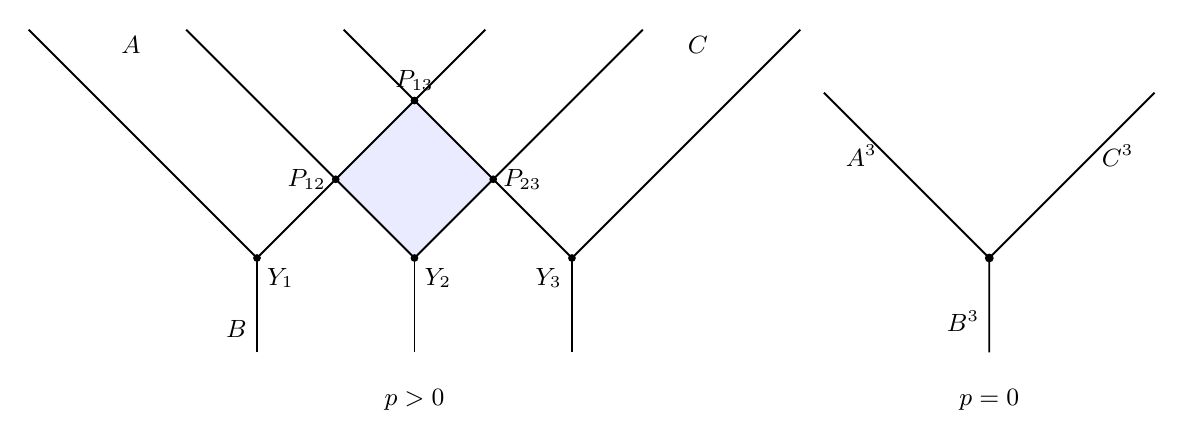
\begin{tikzpicture}[x=2cm,y=2cm,line width=.7pt,
  every node/.style={font=\small},>=Stealth]
  \begin{scope}
    \fill[blue!8] (0,0)--(-.5,.5)--(0,1)--(.5,.5)--cycle;
    \foreach \r in {-1,0,1} {
      \draw (\r,-.6)--(\r,0);
      \draw (\r,0)--({\r-1.45},1.45);
      \draw (\r,0)--({\r+1.45},1.45);
    }
    \foreach \x/\y in {-1/0,0/0,1/0,-.5/.5,.5/.5,0/1}
      \fill (\x,\y) circle (1.4pt);
    \node[below right] at (-1,0) {$Y_1$};
    \node[below right] at (0,0) {$Y_2$};
    \node[below left] at (1,0) {$Y_3$};
    \node[left] at (-.5,.5) {$P_{12}$};
    \node[right] at (.5,.5) {$P_{23}$};
    \node[above] at (0,1) {$P_{13}$};
    \node at (-1.8,1.35) {$A$};
    \node at (1.8,1.35) {$C$};
    \node[left] at (-1,-.45) {$B$};
    \node at (0,-.9) {$p>0$};
  \end{scope}
  \begin{scope}[xshift=7.3cm]
    \draw (0,-.6)--(0,0)--(-1.05,1.05);
    \draw (0,0)--(1.05,1.05);
    \fill (0,0) circle (1.6pt);
    \node[left] at (0,-.4) {$B^3$};
    \node[left] at (-.65,.65) {$A^3$};
    \node[right] at (.65,.65) {$C^3$};
    \node at (0,-.9) {$p=0$};
  \end{scope}
\end{tikzpicture}

\caption{The support of \eqref{eq:diamondweights} for $p>0$
(left) and $p=0$ (right). The left panel uses vertical coordinate
$a t/p$ and horizontal coordinate $x/p$. Its finite core has six
vertices and one bounded diamond. At $p=0$ the entire finite core collapses to
one Y with edge multiplicity three. The four-valent crossings have
vertex objects $A\oplus C$.}
\label{fig:diamondcollapse}
\end{figure}

\begin{proposition}\label{prop:collapsecontinuity}
For all $p,p'\ge0$,
\begin{equation}\label{eq:collapsecontinuity}
 \sup_{t\in\RR}\max_{v=A,C}
 d_2(h_v(t;p),h_v(t;p'))\le\pi\sqrt2\,|p-p'|.
\end{equation}
The same bound holds for each outgoing full boundary norm.
At $p=0$ all three boundary norms are $h_0$, and the support
is the single Y with labels $B^3,A^3,C^3$.
\end{proposition}

\begin{proof}
Since $0<\partial_x\lambda(x,s)\le(1+s^2)^{-1}$,
each integral in \eqref{eq:diamondweights} gives
\[
 |w_{vi}(t;p)-w_{vi}(t;p')|
       \le\pi|r_i(p)-r_i(p')|
\]
uniformly in $t$. The same basis diagonalizes both norms, so
summing the squares of the three weight differences proves
\eqref{eq:collapsecontinuity}. Multiplication by the same
reference scalar is an isometry; taking normalized limits
gives the outgoing bound. At $p=0$, the incoming weights are
zero and the outgoing weights are $A_{\epsilon_va}(t)$.
Normalization removes the latter exactly. This proves the
last assertion and displays the collapse explicitly.
\end{proof}

The estimate proves continuity of the full norm paths through
this particular topology change. It does not establish uniform
continuity for arbitrary boundary triples. Although this example
has a bounded face, its norms are a direct sum of scalar norms;
bounded faces do not require irreducible boundary data.

\subsection{A triple with no common orthogonal splitting}
Fix $u>0$. Give the following three bases the weights $(-2u,-u,0)$:
\begin{equation}\label{eq:irreducibletriple}
 \begin{split}
 b^{(1)}&=(e_1,e_2,e_3),\\
 b^{(2)}&=(e_3,e_2,e_1),\\
 b^{(3)}&=(e_1+e_2+e_3,\ e_1+2e_2+3e_3,\ e_3).
 \end{split}
\end{equation}
Their basis matrices are invertible over $\CC$. Denote the
resulting norms by $h_1,h_2,h_3$ and the standard norm by $h_0$.
They are valid full boundary data $(h_B,h_A^+,h_C^+)$.

We verify that these norms have neither a common apartment nor
a nontrivial common orthogonal direct-sum decomposition.
Each is at most $h_0$. In its residue space the vectors on
which $h_i<h_0$ span the plane generated by the first two
vectors of $b^{(i)}$. These planes are
\[
 P_1=\langle e_1,e_2\rangle,\quad
 P_2=\langle e_2,e_3\rangle,\quad
 P_3=\{x_1-2x_2+x_3=0\}.
\]
Their common intersection is zero. Rescale any nonzero vector
to have $h_0$-norm one, using the full real value group.
Its nonzero residue misses one of the planes, so some $h_i$
has value one on it. Hence $\max_i h_i=h_0$ pointwise.

If the three norms had a common apartment, their maximum
would belong to it too. Reducing a common $h_0$-orthonormal
basis would split all three complete residue flags. The
first two flags are opposite, with canonical intersection
lines $\CC e_1,\CC e_2,\CC e_3$. A basis splitting both
must consist of these lines. The first line of the third
flag is $\CC(e_1+e_2+e_3)$, a contradiction.

More generally, a common orthogonal decomposition would be
orthogonal for $h_0$ and would reduce to a decomposition of
$\CC^3$ splitting the three flags. Its projection preserves
the first two opposite flags, so it is a diagonal idempotent
in the coordinate basis. Preserving the third flag's first
line forces all three diagonal entries to agree. The
projection is therefore zero or identity, and one residue
summand, hence one original summand, is zero. This excludes
a nontrivial decomposition. Theorem~\ref{thm:main} applies
to these triples without reducing them to scalar paths.

\subsection{Full norm information beyond pairwise spectra}
Here is a valued family making that distinction numerical.
Set $u=1$, take $0<s<1$, and put $b=T^s$. Keep the first
two bases in \eqref{eq:irreducibletriple}, and replace the
third by the columns of
\[
 B_3(s)=\begin{pmatrix}1&1&0\\b&2&0\\1&3&1\end{pmatrix}.
\]
Its determinant $2-b$ is a unit. Give all three bases weights
$(-2,-1,0)$. Every pairwise logarithmic relative spectrum is
$(2,0,-2)$, independently of $s$. One can see this from the
exterior minors: after including the norm weights the minimum
valuations of the entries and of the two-by-two minors are
both $-2$, while the determinant valuation is zero. Unit
extremal minors attain these minima; positive-valuation
entries cannot decrease them.

For an explicit three-norm invariant, use the standard volume
form and let $L_i=\{v:h_i(v)\le1\}$. Define
\[
 D_{111}(h_1,h_2,h_3)
   =-\min\{\nu\det(v_1,v_2,v_3):v_i\in L_i\}.
\]
Each lattice has the finite orthonormal generators
$T^{-2}b^{(i)}_1,T^{-1}b^{(i)}_2,b^{(i)}_3$.
Multilinearity and the ultrametric inequality reduce the
minimum to the finitely many choices of one generator from
each lattice. Choosing the first generator in each gives
valuation $-6+s$, because the unscaled determinant is
$\pm b$. Every other choice has weight sum at least $-5$
and an integral determinant. Since $s<1$, the minimum is
$-6+s$, and therefore
\begin{equation}\label{eq:tripleinvariant}
 D_{111}=6-s.
\end{equation}
Thus the pairwise spectra discard information retained by
the full norm triple. The general theorem applies to every
member of this valued family. We do not identify its support
with the diamond above, or with the dual of a numerical hive
built from determinant invariants.


\subsection{Reproducibility}
The accompanying source includes the script
\texttt{check\_examples.py}. It enumerates the nonzero exterior minors of the valued family
and verifies their affine valuation inequalities on the whole
interval $0<s<1$. It also computes the triple determinant
minimum and the rational coordinates, incidence relations and
area of the normalized diamond. Figure~\ref{fig:diamondcollapse}
is drawn directly from those coordinates in the accompanying
TikZ source. The analytic convergence and continuity arguments
are the proofs above and do not depend on quadrature.

\section{The matching condition and further questions}\label{sec:comparison}

\subsection{An edgewise switching example}
The following calculation explains the distinction between the uniqueness
proved here and the edgewise conditions printed in
\cite[Definition~7.8]{HKKP26}. It concerns those displayed conditions;
it is not asserted to define a spectral-network object in the sense of
\cite{HKS24}.

Fix $p>0$, put $r=(-p,0,p)$ and $\tau=3$, and let
$I=(-2,-1)$, $J=(1,2)$. Let $\sigma$ exchange indices $1,3$
and fix $2$. For $L=I$ or $J$ and $t\le\tau$, define
\begin{equation}\label{eq:switchweights}
 w_i^L(t)=\int_{-\infty}^t
 \left[\boldsymbol1_{s\notin L}\lambda(r_i,s)
       +\boldsymbol1_{s\in L}\lambda(r_{\sigma(i)},s)\right]\,\dd s.
\end{equation}
Use these weights at both vertices in the standard basis.
The identity arrow is an isometry and the norms tend to the
same standard incoming norm.

The function $\lambda(p,s)$ is even in $s$. Its integrals over
$I$ and $J$ agree. Since the first and third positions are
opposites and the second is zero, the two sets of weights in
\eqref{eq:switchweights} coincide for $2\le t\le3$.
Write $k_i$ for their common value at $t=\tau$. Continue both
paths by
\[
 w_{vi}(t)=k_i+
   \int_\tau^t\lambda(r_i+\epsilon_va(s-\tau),s)\,\dd s,
 \qquad t\ge\tau.
\]
The coordinate gaps are positive for $t>\tau$, and the
outgoing derivatives agree with the incoming derivatives
at $\tau$. Both normalized outgoing limits exist, by the
same integrable difference estimate as in
\eqref{eq:scalarboundarymap}. Since the paths coincide on
this whole outgoing tail, those full limits are equal.

The two paths are nevertheless different. On $-2<t<-1$,
\[
 w_1^I(t)-w_1^J(t)
       =2\int_{-2}^t\lambda(p,s)\,\dd s>0.
\]
Evaluation on $e_1$ detects their difference as actual norms.
At every regular incoming time the unordered positions of
either path are $\{-p,0,p\}$, with stable $B$ labels.
At each switch the coordinate subspaces carrying those
positions are exchanged. After $\tau$ their supports are
the same three Ys and their crossings, translated in time
from \eqref{eq:diamondvertices}. This finite support is
connected and balanced. Subdivide at the switches and
crossings; all open edges have stable labels and the required
straight directions. At a switch both adjacent abstract
labels are $B$, and numerical charge conservation holds.

At a switch, however, the one-sided coordinate velocity
vectors in the fixed apartment differ. In the $u$ coordinate,
if they are $v^-,v^+$ at a switch $u_0$, then the Euclidean
apartment formula gives
\[
 d_2\bigl(y_v(u_0),\midpt(y_v(u_0-h),y_v(u_0+h))\bigr)
       =\tfrac h2\norm{v^+-v^-}_2+O(h^2).
\]
The coefficient is nonzero. Thus both paths fail
\eqref{eq:matching}. Equality of support, phases, abstract
edge labels and full ends has not identified the embedded
velocity subspaces across the exceptional times.

The printed definition describes an edge label as a graded
object of a velocity filtration. If that phrase is intended
to include additional transport of its embedding, that
transport is precisely what must be specified to exclude
this example. We have made one sufficient intrinsic condition
explicit and proved the correspondence in the resulting
finite regular class. The calculation above does not disprove
an interpretation incorporating stronger categorical gluing.

\subsection{Comparison with categorical networks}
Proposition~\ref{prop:vertexfiltrations} goes from matched norm
paths to local residue objects, two increasing-phase filtrations
and their edge quotients. The reverse implication is a separate
question: which globally framed network data determine opposite
first-order norm germs? In particular, the local existence of
two filtrations of an abstract representation does not by itself
supply the embedded opposition used in
\eqref{eq:vertexdecomposition}.

A comparison with the global Fukaya-category construction would
also have to identify the relevant Novikov-field object and its
gluing data. The uniqueness theorem of
\cite[Theorem~4.15]{HKS24}, in its constant-coefficient,
product-type setting, gives support equality and S-equivalence
of reductions for networks representing the same object after
Novikov extension. It does not supply this comparison or assert
equality of full norm paths. The present variational uniqueness
uses the specified boundary triple and the midpoint condition
directly.

\subsection{Dependence on the boundary data}
Theorem~\ref{thm:main} includes every full split boundary triple,
and hence includes degenerate inputs. General continuity of the
assignment remains open here. A natural topology on triples is
the maximum of the three unnormalized $d_2$ distances. For paths,
one may use uniform vertexwise $d_2$ distance after applying the
same prescribed phase scalars on each end. The estimate in
Proposition~\ref{prop:collapsecontinuity} establishes this
continuity for one explicit family through a bounded-face
collapse. A general result would have to control comparisons
between variational problems with different full reference
norms, rather than only competitors in one fixed-end problem.

Two other extensions are distinct from that continuity problem.
First, the theorem fixes the symmetric $A_2$ charges and radial
area form; its finite-support proof uses the three resulting
monotone directions. Second, uniqueness has been proved among
finite regular paths with matching. Extending it to a larger
intrinsically defined class would require a regularity theorem
for that class or a suitable direct comparison, even though the
minimum itself already has a finite algebraic presentation.


\begin{thebibliography}{HKKP26}

\bibitem[AW13]{AW13}
G.~D.~Appleby and T.~Whitehead, \emph{Matrix pairs over valuation rings
and $\RR$-valued Littlewood--Richardson fillings}, Linear Multilinear
Algebra \textbf{61} (2013), no.~8, 1063--1115,
\href{https://doi.org/10.1080/03081087.2012.731204}{doi:10.1080/03081087.2012.731204}.

\bibitem[AW18]{AW18}
G.~D.~Appleby and T.~Whitehead, \emph{Hives determined by pairs in
the affine Grassmannian over discrete valuation rings}, preprint (2018),
\href{https://arxiv.org/abs/1810.01748}{arXiv:1810.01748}.

\bibitem[BB26]{BB26}
O.~Ben-Bassat, \emph{Harmonic norms on quiver representations over
non-Archimedean fields}, preprint (2026),
\href{https://arxiv.org/abs/2610.01694}{arXiv:2610.01694}.

\bibitem[BE21]{BE21}
S.~Boucksom and D.~Eriksson, \emph{Spaces of norms, determinant of cohomology
and Fekete points in non-Archimedean geometry}, Adv. Math. \textbf{378}
(2021), article~107501, \href{https://doi.org/10.1016/j.aim.2020.107501}{doi:10.1016/j.aim.2020.107501}.

\bibitem[FOOO10]{FOOO10}
K.~Fukaya, Y.-G.~Oh, H.~Ohta and K.~Ono, \emph{Lagrangian Floer theory
on compact toric manifolds I}, Duke Math. J. \textbf{151} (2010), 23--175,
\href{https://doi.org/10.1215/00127094-2009-062}{doi:10.1215/00127094-2009-062};
preprint version \href{https://arxiv.org/abs/0802.1703v3}{arXiv:0802.1703v3}.

\bibitem[HKKP26]{HKKP26}
F.~Haiden, L.~Katzarkov, M.~Kontsevich and P.~Pandit,
\emph{Towards categorical K\"ahler geometry}, preprint (2026),
\href{https://arxiv.org/abs/2609.00978}{arXiv:2609.00978}.

\bibitem[HKS24]{HKS24}
F.~Haiden, L.~Katzarkov and C.~Simpson,
\emph{Spectral networks and stability conditions for Fukaya categories
with coefficients}, Comm. Math. Phys. \textbf{405} (2024), no.~11,
article~264, \href{https://doi.org/10.1007/s00220-024-05138-9}{doi:10.1007/s00220-024-05138-9}.

\bibitem[KT99]{KT99}
A.~Knutson and T.~Tao, \emph{The honeycomb model of $\mathrm{GL}_n(\CC)$
tensor products I: Proof of the saturation conjecture},
J. Amer. Math. Soc. \textbf{12} (1999), no.~4, 1055--1090,
\href{https://doi.org/10.1090/S0894-0347-99-00299-4}{doi:10.1090/S0894-0347-99-00299-4}.

\bibitem[KS97]{KS97}
N.~J.~Korevaar and R.~M.~Schoen, \emph{Global existence theorems for
harmonic maps to non-locally compact spaces}, Comm. Anal. Geom.
\textbf{5} (1997), no.~2, 333--387,
\href{https://doi.org/10.4310/CAG.1997.v5.n2.a4}{doi:10.4310/CAG.1997.v5.n2.a4}.

\bibitem[MPW26]{MPW26}
A.~Moitra, A.~Postnikov and D.~Woodruff,
\emph{Honeycombs and sums of Hermitian matrices, revisited}, preprint
(2026), \href{https://arxiv.org/abs/2607.06710}{arXiv:2607.06710}.

\bibitem[Poo93]{Poonen93}
B.~Poonen, \emph{Maximally complete fields}, Enseign. Math. (2)
\textbf{39} (1993), 87--106.

\bibitem[Yin10]{Yin10}
Y.~Yin, \emph{Quantifier elimination and minimality conditions in
algebraically closed valued fields}, preprint (2010),
\href{https://arxiv.org/abs/1006.1393}{arXiv:1006.1393}.

\end{thebibliography}

\end{document}
